\documentclass{cumcmthesis}
% \documentclass[withoutpreface,bwprint]{cumcmthesis} %去掉封面与编号页,电子版提交的时候使用。
%for long table
\usepackage{longtable}

%for table toprule line
\usepackage{booktabs}

\usepackage{autobreak}
\usepackage[framemethod=TikZ]{mdframed}
\usepackage{url}   % 网页链接
\usepackage{subcaption} % 子标题
\title{无人机编队飞行中的纯方位无源定位模型研究}
\tihao{A}
\baominghao{202227003120}
\schoolname{西北农林科技大学}
\membera{ }
\memberb{ }
\memberc{ }
\supervisor{ }
\yearinput{2020}
\monthinput{08}
\dayinput{22}

\begin{document}

 \maketitle
 \begin{abstract}

针对问题一,此时编队为圆形编队,对第一小问,在知道圆心的一架无人机和圆周上两架发射机的编号的前提下,即已知发射机位置和接收角的前提下计算无人机的位置。通过平面几何基本定理,角的关系和解三角形的相关知识列出方程组,由于方程组中存在超越方程,因此采用图形的方式求得数值解,进而计算出所需定位的无人机位置从而实现定位。

对第二小问,此时仅知FY00和FY01两架飞机,剩余飞机编号未知,即剩余发射机的位置未知。根据几何知识,不共线的三点能确定一个圆,因此表示出所有发射机与接收机所在点所形成的圆轨迹方程,求出多圆交点即可确定接收机的飞机位置。采用依次增加无人机数量的方式。当增加的无人机数量为1时,此时共三架发射机,结果总存在两架对称的可能接收机,因此增加1架无人机无法实现定位。当增加的无人机数量为2时,设接收机位置为M,共4架发射机,共6种组合,舍弃掉不确定的情况有四个组合中每三点建立外接圆。由平面几何知识可知过同一点的确定的四个圆不存在第二个交点,建立出定位模型,利用最小二乘法求解。因此当增加的未知编号的飞机数为2时可以实现接收机的定位。但若注意两架新增的发射机不能对称,否则仍无法对目标无人机进行定位。

对第三小问,圆周上三架未知编号的发射机和FY00可以确定接收机的位置。本问中,对接收机定位时认为发射机是在标准圆周上的,因此定位存在偏差。在此基础上将编队均匀分布到某个圆周上,我们将除FY00外的无人机的极径的平均作为理想圆周的半径。对问题进行分析可得无人机的偏差定位和实际定位与FY00是共线的,通过几何关系求出偏差的定位,将即接收机得知的定位,同时无人机通过期望移动到标准圆周上进行移动,之后换算出移动后的实际位置,与理想圆周的对应位置计算距离,将本轮所有除FY00对理想圆周的距离进行求和作为目标函数。 遍历所有的发射机组合共84种计算出本轮最优的发射机组合,同时将该趟位置作为下一次迭代的初始位置。直到收敛。求得经过仅四次调整后误差大小为2.37e-02,前三次调度的飞机号为1	4 7,3 4 5,3	6 9,理想半径为104.63m。效果优良,收敛迅速。

对问题2,此时编队形状变成了锥形,对无人机的调整方案与问题1的第三小问是相同的,但由于形状的不同,对于偏差的定位存在差异。本问中提出基于最小误差角和的偏差点定位方式。使用matlab进行仿真,初始间距为50m,添加10\%的误差扰动。尝试调度到45m的间距上。经过约10次调整收敛,此时误差为0.9047m。得到了十分满意的效果。



\keywords{无人机\quad  纯方位无源定位\quad   最小二乘法\quad  贪心算法}
\end{abstract}

%目录  2019 明确不要目录,我觉得这个规定太好了
%\tableofcontents

%\newpage

 \section{问题重述}
 \subsection{问题背景}
 无人机是利用无线电遥控设备和自备的程序控制装置操纵的不载人飞机。近年来,无人机在各个领域得到了广泛的应用,如军事、环境监测、影视航拍\cite{22}等,尤其是无人机飞行时保持无线电静默,不被敌方雷达或敌方侦察机探测到在现代国防与战争中有着十分重要的意义。而单个无人机的应用是有限的,为了完成更多的任务,可以采用无人机组,编队飞行提高工作效率。
 
 在编队飞行的过程中,无人机的队形保持\cite{11}是最为基础的部分。无人机集群在遂行编队飞行时,为避免外界干扰,应尽可能保持电磁静默,拟采用纯方位无源定位的方法调整无人机的位置,即由编队中某几架无人机发射信号、其余无人机被动接收信号,从中提取出方向信息进行定位,来调整无人机的位置。在编队飞行中,每一架无人机有固定编号,且各个无人机相对位置保持不变。
\subsection{问题提出}
%\begin{problem}
\textbf{问题一:}10架无人机形成圆形编队,其中九架无人机均匀分布在某一圆周上,另一架无人机位于圆心,且均保持在同一高度上飞行。
%\end{problem}

(1)位于圆心的无人机和编队中另 2 架无人机发射信号,其余位置略有偏差的无人机被动接收信号。当发射信号的无人机位置无偏差且编号已知时,建立被动接收信号无人机的定位模型。

(2)某位置略有偏差的无人机接收到编号为 FY00 和 FY01 的无人机发射的信号,另接收到编队中若干编号未知的无人机发射的信号。若发射信号的无人机位置无偏差,除 FY00 和 FY01外,还需要几架无人机发射信号,才能实现无人机的有效定位?

(3)按编队要求,1 架无人机位于圆心,另 9 架无人机均匀分布在半径为 100 m 的圆周上。当初始时刻无人机的位置略有偏差时,请给出合理的无人机位置调整方案。每次只能选择编号为 FY00 的无人机和圆周上最多 3 架无人机遂行发射信号,仅根据接收到的方向信息来调整无人机的位置,使得 9 架无人机最终均匀分布在某个圆周上。

%\begin{problem}
\textbf{问题二:}实际飞行中,无人机集群也可以是其他编队队形,例如锥形编队队形。仍考虑纯方位无源定位的情形,设计无人机位置调整方案。
%\end{problem}

\section{问题分析}
对于问题一:

问题一让我们针对无人机编队的形状为圆形的情况进行分析和讨论。此时我们假设所有飞机的飞行高度均一致,无人机编队飞行时可将其抽象成质点进行分析与研究。同时,为了方便定义每一架飞机的位置,我们建立了极坐标系与直角坐标系两个坐标系进行下面的分析。对于每架无人机,我们均不考虑其在队形移动时因为速度,偏转角度等对实际模型带来的影响,仅考虑通过无源定位模型进行无人机的调度。

第(1)问:

要求我们在FY00及其他两架位置无偏差的无人机进行信号发射且接收机能够知道发射机编号的前提下对其他无人机进行位置定位。由于接收机知道发射机的信号,故可精确的根据角度及半径R进行解三角形的处理,利用接收到的三个方向角进行当前位置的定位。所需要注意的是,由于解三角形时三角函数确定正负但并不能确定其所在象限,所以我们要对其进行分类讨论得到最后的定位结果。

第(2)问:

问题一(2)要求我们求解除FY00,FY01以外还需要几架无人机能在发射机位置无偏差、接收机不知道发射机编号的情况下对接收机进行准确的定位。首先我们根据圆的对称性规则得出以下结论:在只增添一架飞机的时候我们会有两架相对于x轴对称的无人机不能进行准确的定位,所以开始对增加两架飞机的情况进行分析。

首先,我们考虑FY00,FY01,A1,A2与接收机M’可能形成的夹角组合一共有 种可能,通过对方程次数以及方程组同构现象的分析最终确定了三组夹角。根据几何知识可知三点可以唯一确定一个圆,且由于三点中包含点M’,所以可以表示出四个M’的圆轨迹方程,这四个圆的共同交点即为M’。所以我们可以通过方程组求解出M’的坐标。但是我们考虑到如果选择关于x轴对称的两架飞机时,无法对其他的关于x轴对称的两架无人机进行准确的定位区别。所以得出的结论是再加两架飞机即可进行定位,但是所选的这两架飞机不能关于x轴对称。

第(3)问:
需要考虑在除了编号为FY00的无人机以外其他9架无人机位置均有偏差的情况下选择从外面9架飞机中选择3架无人机进行定位与调整。根据题目所给数据,可以观察到其余 9 架无人机和FY00的距离各有不同,因此可以把 FY01-¬FY09无人机的位置看作是有偏差的,且当有偏差的无人机发射信号时,待接收信号无人机会按照有偏差的方向信息进行位置 调整,最终会调整到一个有偏差的位置,也称为为错误理想位置。在计算的过程中,每一次调整的依据都是通过贪心算法选择总体误差最小的发射机组合进行迭代。所选择的理想半径是在动态调度过程中根据总体误差最小这个前提进行实时调整的,最终满足无人机均匀分布且在同一个圆周上。

对于问题二:

问题二要求我们对第一问所分析出的模型进行推广,我们考虑的推广模型为锥形。为了研究方便,我们以 作为直角坐标系x轴的正半轴进行分析。根据模型一,我们首先对锥形分布的前提下为了进行准确定位与调整所需要的无人机架数进行讨论与分析。我们对标准情况下的无人机坐标给予随机值进行偏移形成我们的初始模型。并对增加三架无人机的一般定位与模型方案进行计算,要求根据无源定位使得有偏差的无人机群通过调整回到锥形队列中。目标函数与问题一(3)一致,所需调整的仅有约束条件,最后得出调整方案
\section{模型假设}
1.假设无人机的位置偏差不包含高度偏差

2.无人机体积小,相对距离远,可以将其看作质点

3.假设在编队飞行中无人机与无人机的相对位置关系保持不变

4.假设发射信号无人机不存在发射故障情况

5.假设发射信号的无人机在结束发射前不会移动

6.假设所有待接收信号的无人机的移动是并行的

7.假设无人机在调整位置时,忽略移动时间
\section{符号说明}
\begin{center}
	\begin{tabular}{cc}
		\toprule[1.5pt]
		\makebox[0.3\textwidth][c]{符号}	&  \makebox[0.4\textwidth][c]{意义} \\ \hline
		$\rho_i$	    & 编号为i的无人机距离中心点的距离 \\ \hline
		$p_i^T$	    & 编号为i的无人机的理想位置 \\ \hline
		$p_i^{FI}$	    & 编号为i的无人机的计算出的错误理想位置 \\ \hline
		$p_i^R$	    & 编号为i的无人机实际位置 \\ \hline
		$p_i^{R'}$	    & 编号为i的无人机移动后的实际位置 \\ \hline
		$p_i^C$	    & 编号为i的无人机的计算位置 \\ \hline
		$\vec{p_D}$ & 无人机移动的位移差\\ 
		 \bottomrule[1.5pt]
	\end{tabular}
\end{center}

\section{模型的建立与求解}

\subsection{问题一第(1)问的模型建立与求解}
\subsubsection{被动接收信号无人机的定位模型}
\begin{figure}[!h]
	\centering
	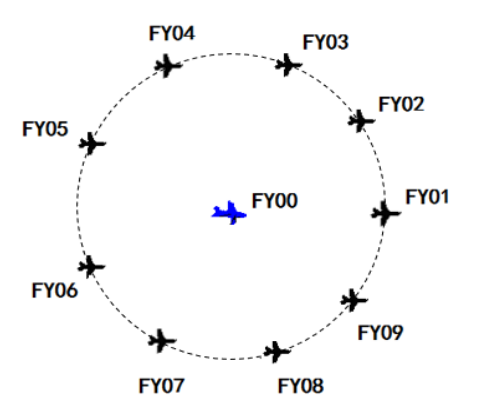
\includegraphics[width=.4\textwidth]{p0}
	\caption{圆形无人机编队示意图}
	\label{fig:p0}
\end{figure}
根据题目,圆形编队队形如\cref{fig:p0}示,因无人机高度一定,我们将其转换为二维平面,以无人机FY00为极点,FY01为极轴,建立极坐标系,如\cref{fig:p1}所示。
\begin{figure}[!h]
	\centering
	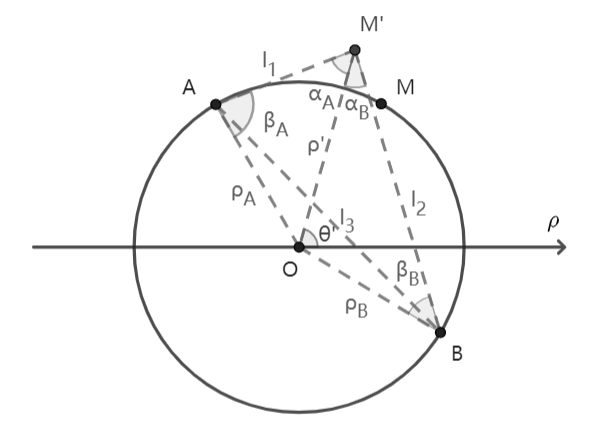
\includegraphics[width=.5\textwidth]{p1}
	\caption{圆形无人机编队极坐标几何关系图}
	\label{fig:p1}
\end{figure}
	设$M'(\rho',\theta')$为位置有偏差的无人机,位于第一象限,其标准位置为$M(\rho,\theta)$,$A(\rho_A,\theta_A)$、$B(\rho_B,\theta_B )$表示另外两架位于圆周上的无人机,位于以OM'两侧。其余分布情况与此情况类似,不做赘述。
	

对于$\triangle BOM'$,由正弦定理得:
	\begin{equation}
		\rho_{A} \sin\beta_{B} = \rho' \sin\alpha_{B}
		\label{eq:1}
	\end{equation}

由内角和关系得:
	\begin{equation}
	\alpha_{B}+ \min \left\{ \theta_{B} - \theta',\left[2\pi - (\theta_{B} - \theta') \right] \right\}    + \beta_{B} = \pi
	\label{eq:2}
	\end{equation}
当$\theta_{B} - \theta' \le \pi$时,公式\cref{eq:2}为$\alpha_{B}+  \theta_{B} - \theta'  + \beta_{B} = \pi$;当$\theta_{B} - \theta' > \pi$时,公式\cref{eq:2}为$\alpha_{B}+  2\pi - (\theta_{B} - \theta')  + \beta_{B} = \pi$

对于$\triangle AOM'$,由正弦定理得:
\begin{equation}
	\rho_{B} \sin\beta_{A} = \rho' \sin\alpha_{A}
	\label{eq:3}
\end{equation}

由内角和关系得:
\begin{equation}
	\alpha_{A}+ \min \left\{ \theta_{A} - \theta',\left[2\pi - (\theta_{A} - \theta') \right] \right\}    + \beta_{A} = \pi
	\label{eq:4}
\end{equation}
当$\theta_{A} - \theta' \le \pi$时,公式\cref{eq:4}为$\alpha_{A}+  \theta_{A} - \theta'  + \beta_{A} = \pi$;当$\theta_{A} - \theta' > \pi$时,公式\cref{eq:4}为$\alpha_{A}+  2\pi - (\theta_{A} - \theta')  + \beta_{A} = \pi$

已知点M、A、B所代表的无人机均位于同一圆周上,即
\begin{equation}
	\rho_{A} = \rho_{B} =\rho
	\label{eq:5}
\end{equation}
因此,根据公式\cref{eq:1}~\cref{eq:5},被动接收信号无人机的定位模型为
\begin{equation}
	\begin{cases}
		\rho_{A} \sin\beta_{B} = \rho' \sin\alpha_{B}\\
		\alpha_{B}+ \min \left\{ \theta_{B} - \theta',\left[2\pi - (\theta_{B} - \theta') \right] \right\}    + \beta_{B} = \pi \\
		\rho_{B} \sin\beta_{A} = \rho' \sin\alpha_{A}\\
		\alpha_{A}+ \min \left\{ \theta_{A} - \theta',\left[2\pi - (\theta_{A} - \theta') \right] \right\}    + \beta_{A} = \pi\\
		\rho_{A} = \rho_{B} =\rho\
	\end{cases}
		\label{eq:10}
\end{equation}
\subsubsection{模型求解}
因为无人机AB的位置不固定,其角的关系也有相应的变化,所以需要分情况讨论$\theta_{A}$与$\theta_{B}$。根据公式\cref{eq:2} \cref{eq:4},$\beta_{A}$的值共有四种情况:
\begin{equation}
	\beta_{A} =
	\begin{cases}
		\alpha_{B}+\theta_{B}+\beta_{B}-\alpha_{A}-\theta_{A} &, \theta_{B}-\theta' \le pi \text{且} \theta_{A}-\theta' \le pi  \\
		\theta_{A}-(\alpha_{B}+\theta_{B}+\beta_{B}+\alpha_{A}) &, \theta_{B}-\theta' \le pi \text{且} \theta_{A}-\theta' > pi  \\
		\theta_{B}-(\alpha_{B}+\theta_{A}+\beta_{B}+\alpha_{A}) &, \theta_{B}-\theta' > pi \text{且} \theta_{A}-\theta' \le pi  \\
		\theta_{A}-\theta_{B}+\alpha_{B}+\beta_{B}-\alpha_{A} &, \theta_{B}-\theta' > pi \text{且} \theta_{A}-\theta' > pi  \\
	\end{cases}
	\label{eq:6}
\end{equation}

由公式\cref{eq:1}\cref{eq:2}\cref{eq:5}得:
\begin{equation}
	\sin \beta_{A} = \frac{\sin \alpha_{A}}{\sin \alpha_{B}} \sin \beta_{B}
	\label{eq:10}
\end{equation}
由反三角函数解得:
\begin{equation}
\beta_{A} = \arcsin \frac{\sin \alpha_{A}}{\sin \alpha_{B}} \sin \beta_{B}
	\label{eq:8}
\end{equation}
易知$\beta_{A} \in (0,\pi),\beta_{B} \in (0,\pi)$
由公式\cref{eq:6}\cref{eq:8}可求得$\beta_{B}$,但显然没有解析解,可以通过曲线相交求得数值解

由公式\cref{eq:1}\cref{eq:2}\cref{eq:5}得:
\begin{equation}
	\begin{aligned}
	&\rho'=\rho \frac{\sin \beta_{B}}{\sin \alpha_{B}} 
	\\
	&\theta'=
		\begin{cases}
		\pi-\alpha_{B}+\theta_{B}-\beta_{B} &, 0< \theta'-\theta_{B}  \le \pi  \\
		\theta_{B}-\alpha_{B}-\beta_{B}-\pi &, \pi< \theta'-\theta_{B}  \le 2pi  \\
		\end{cases}
	\end{aligned}
	\label{eq:9}
\end{equation}
此为待接收信号无人机的位置极坐标。

\subsection{问题一第(2)问的模型建立与求解}
\subsubsection{模型建立}
首先考虑还需要一架发射信号的无人机情况:
\begin{figure}[!h]
	\centering
	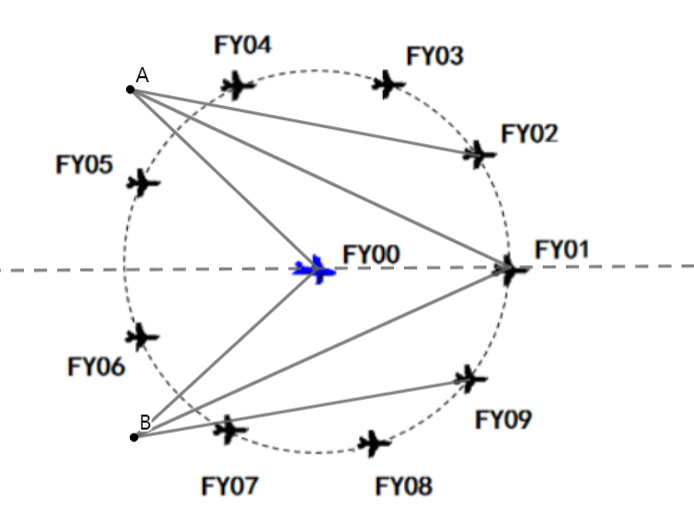
\includegraphics[width=.4\textwidth]{p2}
	\caption{基于三架无人机发射信号定位图}
	\label{fig:p2}
\end{figure}

如图\cref{fig:p2}所示,假设待接收信号无人机位于A点,发射信号飞机已知为FY00,FY01,因不知道第三架发射信号飞机的编号,所以对于待接收信号飞机来说,存在B点使无人机接收到的方位信息与在A点时相同,因此待接收信号无人机并不能确定它自身是在A点还是B点。因此此情况不成立。

然后考虑还需要两架发射信号的无人机情况:

1.当两架无人机关于FY00和FY01所在直线对称时,如\cref{fig:p4}所示,假设待接收信号无人机位于A点,发射信号飞机已知为FY00,FY01,若第三、四架无人机编号为{FY02,FY09}或{FY03,FY08}或{FY04,FY07}或{FY05,FY06},对于待接收信号无人机来说,与上述情况相同,A,B点无人机接收到的方位信息相同,无法进行有效定位,此情况不成立。
\begin{figure}[H]
	\centering
	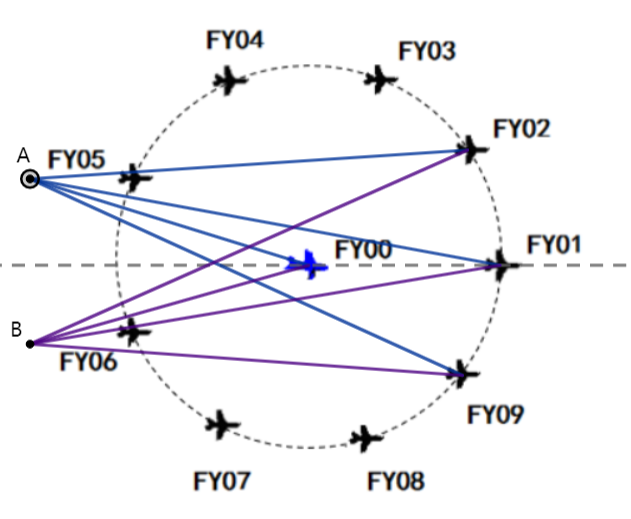
\includegraphics[width=.4\textwidth]{p4}
	\caption{基于四架无人机发射信号定位图}
	\label{fig:p4}
\end{figure}

2.当两架无人机关于FY00和FY01所在直线不对称时:

以无人机FY00为原点,原点到FY01为X轴正方向,建立直角坐标系。
设$M'(x,y)$为待接收信号的无人机,$A_1 A_2$为新增加发射信号无人机,无人机FY00与FY01的距离为R,则无人机的坐标为$FY00(0,0)$,$FY01(R,0)$,$A_1(Rcos(k_1\alpha),Rsin(k_1\alpha))$,$A_2(Rcos(k_2\alpha),$ $Rsin(k_2\alpha))$,其中$k_1 k_2\text{为常数,且}k_1 \ne -k_2\alpha=\frac{2}{9} \pi$。
根据几何知识,不在同一直线的三点能确定一个圆,因此表示出所有信号发射飞机与M'点所形成的圆轨迹方程,求出多圆交点即可确定待接收信号的飞机位置。

圆中三点选取有六种组合,分别为:$(1)FY00,FY01,M';(2)FY00,A_1,M';(3)FY00,$ $A_2,M'(4)FY01,A_1,M';(5)FY01,A_2,M';(6)A_1,A_2,M'$。
其中,组合(6)的圆方程式中会同时包含$k_1,k_2$两个未知数,无法求解,故不考虑此组合;组合(2)(3)的圆方程式所差参数由$A_1A_2$决定,会出现同构情况。因此只考虑(1)(3)(4)(5)组合,如\cref{fig:p3}所示:
\begin{figure}[H]
	\centering
	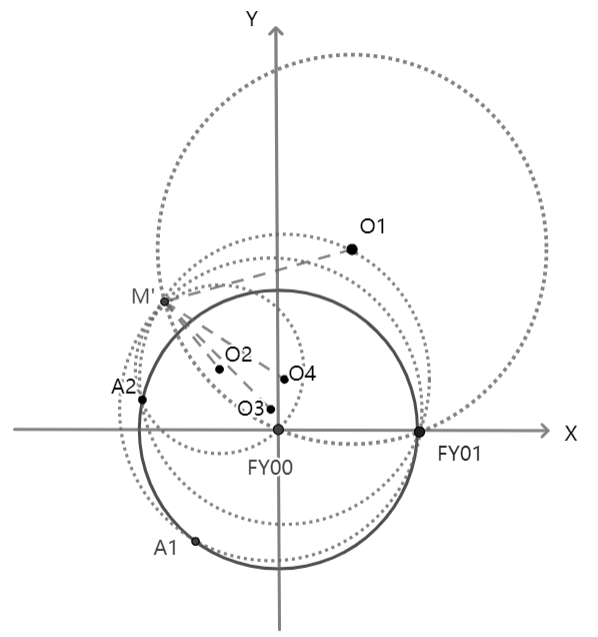
\includegraphics[width=.6\textwidth]{p3}
	\caption{无人机定位模型示意图}
	\label{fig:p3}
\end{figure}
设圆方程的圆心为$O_i(x_i,y_i)$,半径为$r_i$,$\alpha_i$为M'接收到其余两架无人机发送信号的方位信息角,$i = 1,2,3,4$分别对应组合(1)(3)(4)(5)所构建的圆。其方程为:
\begin{equation}
	(x-x_i)^2+(y-y_i)^2=r_i^2,i=1,2,3,4
	\label{eq:14}
\end{equation}
则圆$O_1$必过FY00(0,0),FY01(R,0)两点。且根据圆上弦所对的圆周角度数相等及垂径定理可得方程组:
\[
%\begin{equation}
	\begin{cases}
		x_1^2+y_1^2=r_1^2\\
		(x_1-R)^2+y_1^2=r_1^2\\
		R^2=4r_1\sin\alpha_{1}\\
	\end{cases}
	\label{eq:11}
%\end{equation}
\]
同理可得到其余圆方程组:
\[
%\begin{equation}
	\begin{cases}
		x_2^2+y_2^2=r_2^2\\
		(x_2-R\cos k_2 \alpha)^2+(y_2-R\sin k_2 \alpha)^2=r_2^2\\
		R_1^2=4r_2\sin\alpha_2\\
	\end{cases}
	\label{eq:12}
%\end{equation}
\]
\[
%\begin{equation}
	\begin{cases}
		(x_3-R)^2+y_3^2=r_3^2\\
		(x_3-R\cos k_1 \alpha)^2+(y_3-R\sin k_1 \alpha)^2=r_3^2\\
		(R-R\cos k_1 \alpha)^2+(1-R\sin k_1 \alpha)^2=2r_3^2 \sin^2 \alpha_3\\
	\end{cases}
	\label{eq:13}
%\end{equation}
\]
\[
%\begin{equation}
	\begin{cases}
		(x_4-R)^2+y_4^2=r_4^2\\
		(x_4-R\cos k_2 \alpha)^2+(y_4-R\sin k_2 \alpha)^2=r_4^2\\
		(R-R\cos k_2 \alpha)^2+(1-R\sin k_2 \alpha)^2=2r_4^2 \sin^2 \alpha_4\\
	\end{cases}
	\label{eq:15}
%\end{equation}
\]
解得:
\begin{equation}
	\begin{cases}
		r_1=\frac{R}{2\sin \alpha_1}\\
		x_1=\frac{R}{2}\\
		y_1=\frac{R}{2\tan \alpha_1}\\
	\end{cases}
	\label{eq:16}
\end{equation}
\begin{equation}
	\begin{cases}
		r_2=\frac{R}{2\sin \alpha_2}\\
		x_2=\frac{R}{2\cos k_2 \alpha}-y_2 \tan k_2\alpha \\
		y_2=\frac{R\sin k_2 \alpha}{2} +\sqrt{ \frac{R^2 \sin^2 k_2 \alpha}{4} - r_2^2cos^2 k_2 \alpha}\\
	\end{cases}
	\label{eq:17}
\end{equation}
\begin{equation}
	\begin{cases}
		r_3=\frac{\sqrt{R^2(2-cos k_1 \alpha)^2 + (1-R\sin k_1 \alpha )}}{2\sin \alpha_3}\\
		x_3=\frac{R}{1+\frac{(2\sin^2 k_1 \alpha)^2}{\sin^2 k_1 \alpha}}+ \sqrt{\frac{R^2}{1+\frac{(1-\cos k_1 \alpha)^2}{\sin^2 k_1 \alpha}}-\frac{R_1^2}{1+\frac{1-\cos^2 k_1 \alpha}{\sin^2 k_1 \alpha}}}\\
		y_3=\frac{1-\cos k_1 \alpha}{\sin k_1 \alpha} x_3\\
	\end{cases}
	\label{eq:18}
\end{equation}
\begin{equation}
	\begin{cases}
		r_4=\frac{\sqrt{R^2(2-cos k_2 \alpha)^2 + (1-R\sin k_2 \alpha )}}{2\sin \alpha_3}\\
		x_4=\frac{R}{1+\frac{(2\sin^2 k_2 \alpha)^2}{\sin^2 k_2 \alpha}}+ \sqrt{\frac{R^2}{1+\frac{(1-\cos k_2 \alpha)^2}{\sin^2 k_2 \alpha}}-\frac{R_2^2}{1+\frac{1-\cos^2 k_2 \alpha}{\sin^2 k_2 \alpha}}}\\
		y_4=\frac{1-\cos k_2 \alpha}{\sin k_2 \alpha} x_3\\
	\end{cases}
	\label{eq:19}
\end{equation}

综上,式\cref{eq:14}\cref{eq:16}\cref{eq:17}\cref{eq:18}\cref{eq:19}为对于无人机M'的定位模型
%,满足以下四个圆方程组:
%\begin{equation}
%	\begin{cases}
%		(x-x_1)^2+(y-y_1)^2=r_1^2\\
%		(x-x_2)^2+(y-y_2)^2=r_2^2\\
%		(x-x_3)^2+(y-y_3)^2=r_3^2\\
%		(x-x_4)^2+(y-y_4)^2=r_4^2
%	\end{cases}
%	\label{eq:20}
%\end{equation}

\subsubsection{模型求解}
在这里,采用最小二乘法对模型进行求解。
将各个圆方程相减,可得其矩阵形式:
%\begin{equation}
%	\begin{cases}
%		2(x_2-x_1)x+2(y_2-y_1)y = r_1^2-r_2^2 -(x_1^2+y_1^2)+(x_2^2+y_2^2)\\
%		2(x_3-x_2)x+2(y_3-y_2)y = r_2^2-r_3^2 -(x_2^2+y_2^2)+(x_3^2+y_3^2)\\
%		2(x_4-x_3)x+2(y_4-y_3)y = r_3^2-r_4^2 -(x_3^2+y_3^2)+(x_4^2+y_4^2)
%	\end{cases}
%	\label{eq:20}
%\end{equation}
\begin{equation}
	\mathbf{AX}=\mathbf{B}
	\label{eq:20}
\end{equation}
其中,
\[
\mathbf{A} = \left(
\begin{array}{cc}
	2(x_2-x_1)x & 2(y_2-y_1)y \\
	2(x_3-x_2)x & 2(y_3-y_2)y \\
	2(x_4-x_3)x & 2(y_4-y_3)y\\
\end{array} \right)
\mathbf{X} = \left(
\begin{array}{c}
	x   \\
	y  \\
\end{array} \right)
\mathbf{B} = \left(
\begin{array}{cc}
	r_1^2-r_2^2 -(x_1^2+y_1^2)+(x_2^2+y_2^2)   \\
	r_2^2-r_3^2 -(x_2^2+y_2^2)+(x_3^2+y_3^2)   \\
	r_3^2-r_4^2 -(x_3^2+y_3^2)+(x_4^2+y_4^2)  \\
\end{array} \right)
\]

设误差向量为:\[\epsilon=\mathbf{AX}-\mathbf{B}\]其误差平方和为\[E=|\epsilon|^2=\epsilon^T \epsilon=(\mathbf{AX}-\mathbf{B})^T(\mathbf{AX}-\mathbf{B}) \]

要使得误差最小,即使得E最小,则对E进行求导:
\[\frac{dE}{d\mathbf{X}}=2\mathbf{A}^T\mathbf{A}\mathbf{X}-2\mathbf{A}^T\mathbf{B}=0\]
解得:
\begin{equation}
	\mathbf{X}=(\mathbf{A}^T\mathbf{A})^{-1}(\mathbf{A}^T\mathbf{B})
	\label{eq:21}
\end{equation}
由于M'坐标只有一个,故可以消去$k_1,k_2$得到唯一解。所以仅需新增两架无人机即可完成有效定位

\subsection{问题一第(3)问的模型建立与求解}
\subsubsection{无人机一次移动前后极角变化情况}



在无人机的调度过程中,改变的参数为距离中心点的距离$\rho$和极角$\theta$。首先我们需要讨论一下极角的变化情况,假设无人机移动前后极角不变。
\begin{figure}[!h]
	\centering
	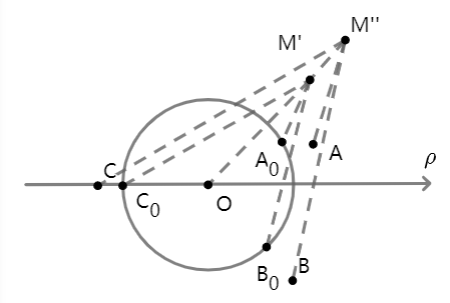
\includegraphics[width=.5\textwidth]{p5}
	\caption{有偏差无人机移动前后几何关系图}
	\label{fig:p5}
\end{figure}

以无人机FY00为极点,FY01为极轴,建立极坐标系,如\cref{fig:p5}所示。设$M''(\rho'',\theta'')$为待接收信号无人机位置,$M'(\rho',\theta')$为待接收信号无人机移动后位置,$A(\rho_A,\theta_{A}),B(\rho_{B},\theta_B),$$C(\rho_C,\theta_C)$为三架发射信号无人机。$A_0(\rho,\theta_A^0),B_0(\rho,\theta_B^0),C_0(\rho,\theta_C^0)$为$A,B,C$无人机的原本位置。
\begin{proof}
	证明$OM'M''$共线。
	
	$\alpha_{A}\text{为}\angle OM''A\text{,}\alpha_{B}\text{为}\angle OM''B\text{,}\alpha_{C}\text{为}\angle OM''C\text{。}$连接$OM''$,过$B$作$B'M''$的平行线交$OM''$直线于点$M'$,连接$M'A^0,M'C^0$。
	我们要
	由同位角关系,显然有:
	\[\angle OM'A^0=\angle OM''A=\alpha_{A}\]
	\[\angle OM'B^0=\angle OM''B=\alpha_{B}\]
	\[\angle OM'C^0=\angle OM''C=\alpha_{C}\]
	
	该点$M'$满足$M''$所处的无人机计算点的要求,即获得的三个角度是由各个发射信号的无人机处在原本位置(标准圆)上时发射的。
	\label{prf:example}
\end{proof}
\begin{lemma}
	三个圆的交点至多存在两个。
	\label{lem:1}
\end{lemma}
\begin{proof}
在平面几何中有且只有一个点$M'$满足上述条件


当点$OA^0M'$不共线时,即发射信号的无人机与接收信号的无人机不相同时,显然成立。
同理,点$OB^0M'$不共线且$OC^0M'$不共线。

作$OA^0M',OB^0M',OC^0M'$的外接圆,分别为$\odot A,\odot B,\odot C$

显然该三个圆存在两个交点$O$和$M'$。由\cref{lem:1}得不存在第三个点使得三圆相交,即不存在别的$M$点使得$\angle OMA^0=\alpha_{A},\angle OMB^0=\alpha_{B},\angle OMC^0=\alpha_{C}$,因此$M'$唯一。

\end{proof}

由证明12知,无人机移动前后极角不变
\subsubsection{基于偏差的无人机定位调度模型}


根据题目所给数据,FY00-FY10无人机的初始位置如所示。可以观察到其余9架无人机和FY00的距离各有不同,因此可以把FY01-FY10无人机的位置看作是有偏差的,且当有偏差的无人机发射信号时,待接收信号无人机会按照有偏差的方向信息进行位置调整,最终会调整到一个有偏差的位置,也称为为错误理想位置。

因此,无人机调度方案的目标函数是使总偏差最小,即无人机根据方向信息调整后的实际位置与我们希望的理想位置的实际距离最小。
\begin{equation}
	\min \sum_{i=1}^{n} || p_i^{R'} - p_i^t||^2
	\label{eq:22}
\end{equation}

理想位置为:
\begin{equation}
	p_i^T=(\frac{1}{n} \sum_{i=1}^{n}    \rho_i,(i-1)\frac{2}{9} \pi)
	\label{eq:23}
\end{equation}
\begin{figure}[!h]
	\centering
	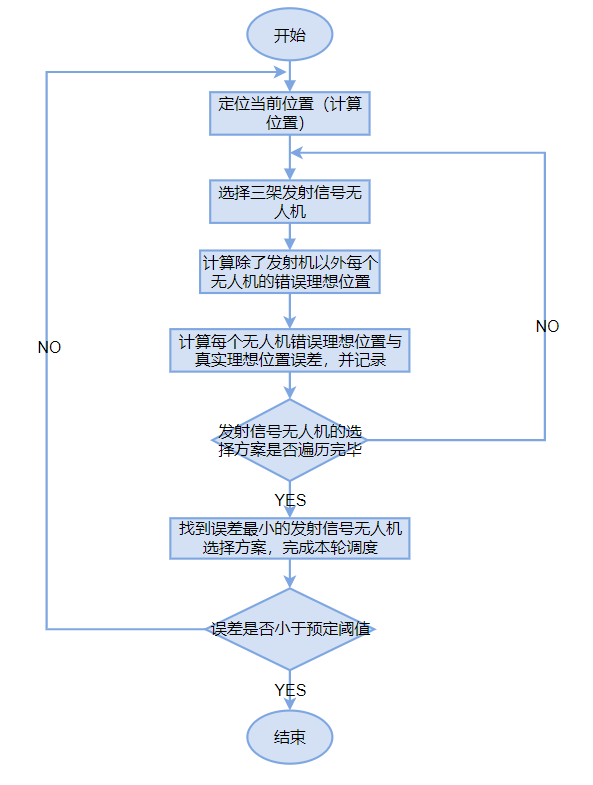
\includegraphics[width=.65\textwidth]{p6}
	\caption{无人机调度流程图}
	\label{fig:p6}
\end{figure}
具体调度流程如\cref{fig:p6}所示:



\textbf{step1} 定位当前位置,把当前位置作为计算位置,即
\begin{equation}
	p_i^C=p_i^R
	\label{eq:24}
\end{equation}
其中,当前位置为$p_i^R=(\rho',\theta')=(\rho',\theta'')$

如\cref{fig:p5}所示,
\[\angle k= \pi - ((\theta_B^0- \theta)+ \alpha_{1})\]
在$\triangle B^0M'O$中,
\[\frac{\rho}{\sin \alpha_1}=\frac{\rho'}{\sin \angle k} \]
解得:
\begin{equation}
	\rho'=\frac{\sin(\min{2\pi-(\theta_B^0-\theta),\theta_B^0-\theta}+ \alpha_1)}{\sin \alpha_1} \rho=\frac{\sin(\min{2\pi-(\theta_B-\theta),\theta_B-\theta}+ \alpha_1)}{\sin \alpha_1} \rho
	\label{eq:25}
\end{equation}
其中,$\theta_{B}=i_B \frac{2}{9}\pi (i_A=1,2,\cdots,9)$

\textbf{step2} 计算每个无人机错误理想位置$p_i^{FI}$,得到位移差
\begin{equation}
	\vec{p_D}=p_i^{FI}-p_i^C
	\label{eq:26}
\end{equation}
\begin{equation}
	\vec{p_i^{R'}}=	\vec{p_i^R}+\vec{p_D}
	\label{eq:27}
\end{equation}

\textbf{step3} 根据公式\cref{eq:22}\cref{eq:26}\cref{eq:27}计算与真实理想的误差

\textbf{step4}选择误差最小的发射信号无人机选择方案进行本轮调度

\textbf{step5}重复step1-step4,直到误差小于预定阈值,本题的模型精度为1e-6

\subsubsection{模型求解}
我们选择贪心算法进行模型的求解。贪心算法,在求解过程的每一步中都采取在当前状态下看来是最好或最优的选择,从而希望最终的结果是最好或最优的。

求解步骤:

1. 将原问题分解成若干轮的无人机移动子问题

2. 对每一子问题分别求解,计算子问题中所有发射信号无人机选择方案及移动误差

3. 得到所有子问题的局部最优解。即在第i轮移动时,得到在当前位置下,最佳的发射信号无人机选择方案及移动结果

4.从初始解出发,不断迭代轮数,得到原问题的全局最优解

初始条件下的模拟结果如\cref{tab:1}所示,选出第一轮总误差最小的发射信号无人机方案:FY01,FY04,FY07
\begin{table}[!htbp]
	\caption{第一轮模拟结果}\label{tab:1} \centering
	\begin{tabular}{cccccc}
		\toprule[1.5pt]
		模拟次数 & 无人机方案 & FY01误差 & $\cdots$ & FY09误差 & 总误差\\
		\midrule[1pt]
		1 & FY01,FY02,FY03 & 4.44444 & 	$\cdots$ & 4.44444 & 45.1239\\
		2 & FY01,FY02,FY04 & 4.44444 & 	$\cdots$ &4.44444&38.2773 \\
		3 & FY01,FY02,FY05 & 4.44444 & 	$\cdots$ & 6.87147& 56.4034\\
		$\cdots$ & $\cdots$ & $\cdots$ & $\cdots$ & $\cdots$ & $\cdots$\\
		84 & FY08,FY09,FY07 & 0.525494 & 	$\cdots$ & 7.57402& 17.5103\\
		\bottomrule[1.5pt]
	\end{tabular}
\end{table}

通过matlab模拟多轮进行求解,得到发射信号无人机的选择方案如\cref{tab:2}所示。

那么无人机的调整方案为:根据\cref{tab:2}进行发射信号无人机的选择,其余无人机接收方位信息进行调整,进行九轮迭代,即可停止,此时误差精度<1e-6,无人机调整完毕的位置见附录\cref{tab:3},与初始位置进行对比如\cref{fig:p-7}所示:
	
\begin{table}[H]
	\caption{发射信号无人机的选择方案}\label{tab:2} \centering
	\begin{tabular}{ccccc}
		\toprule[1.5pt]
		调整次数 &  & 无人机方案 &  & 总误差 \\
		\midrule[1pt]
		1 & FY01 & FY04 & FY07 & 10.2791\\
		2 & FY03 & FY04 & FY05 & 4.59416\\
		3 & FY03 & FY06 & FY09 & 0.415374\\ 
%		4 & FY02 & FY05 & FY09 & 0.023668\\
%		5 & FY01 & FY07 & FY08 & 0.002855\\
%		6 & FY02 & FY03 & FY09 & 0.000218\\
%		7 & FY02 & FY05 & FY07 & 0.000056\\
%		8 & FY03 & FY04 & FY06 & 4.29283E-06\\
%		9 & FY01 & FY06 & FY07 & 8.61033E-07\\
		$\cdots$ & $\cdots$ & $\cdots$ & $\cdots$ & $\cdots$ \\
		20 & FY02 & FY08 & FY09 & 1.24368E-13\\
		\bottomrule[1.5pt]
	\end{tabular}
\end{table}	
%\begin{figure}[H]
%	\centering
%	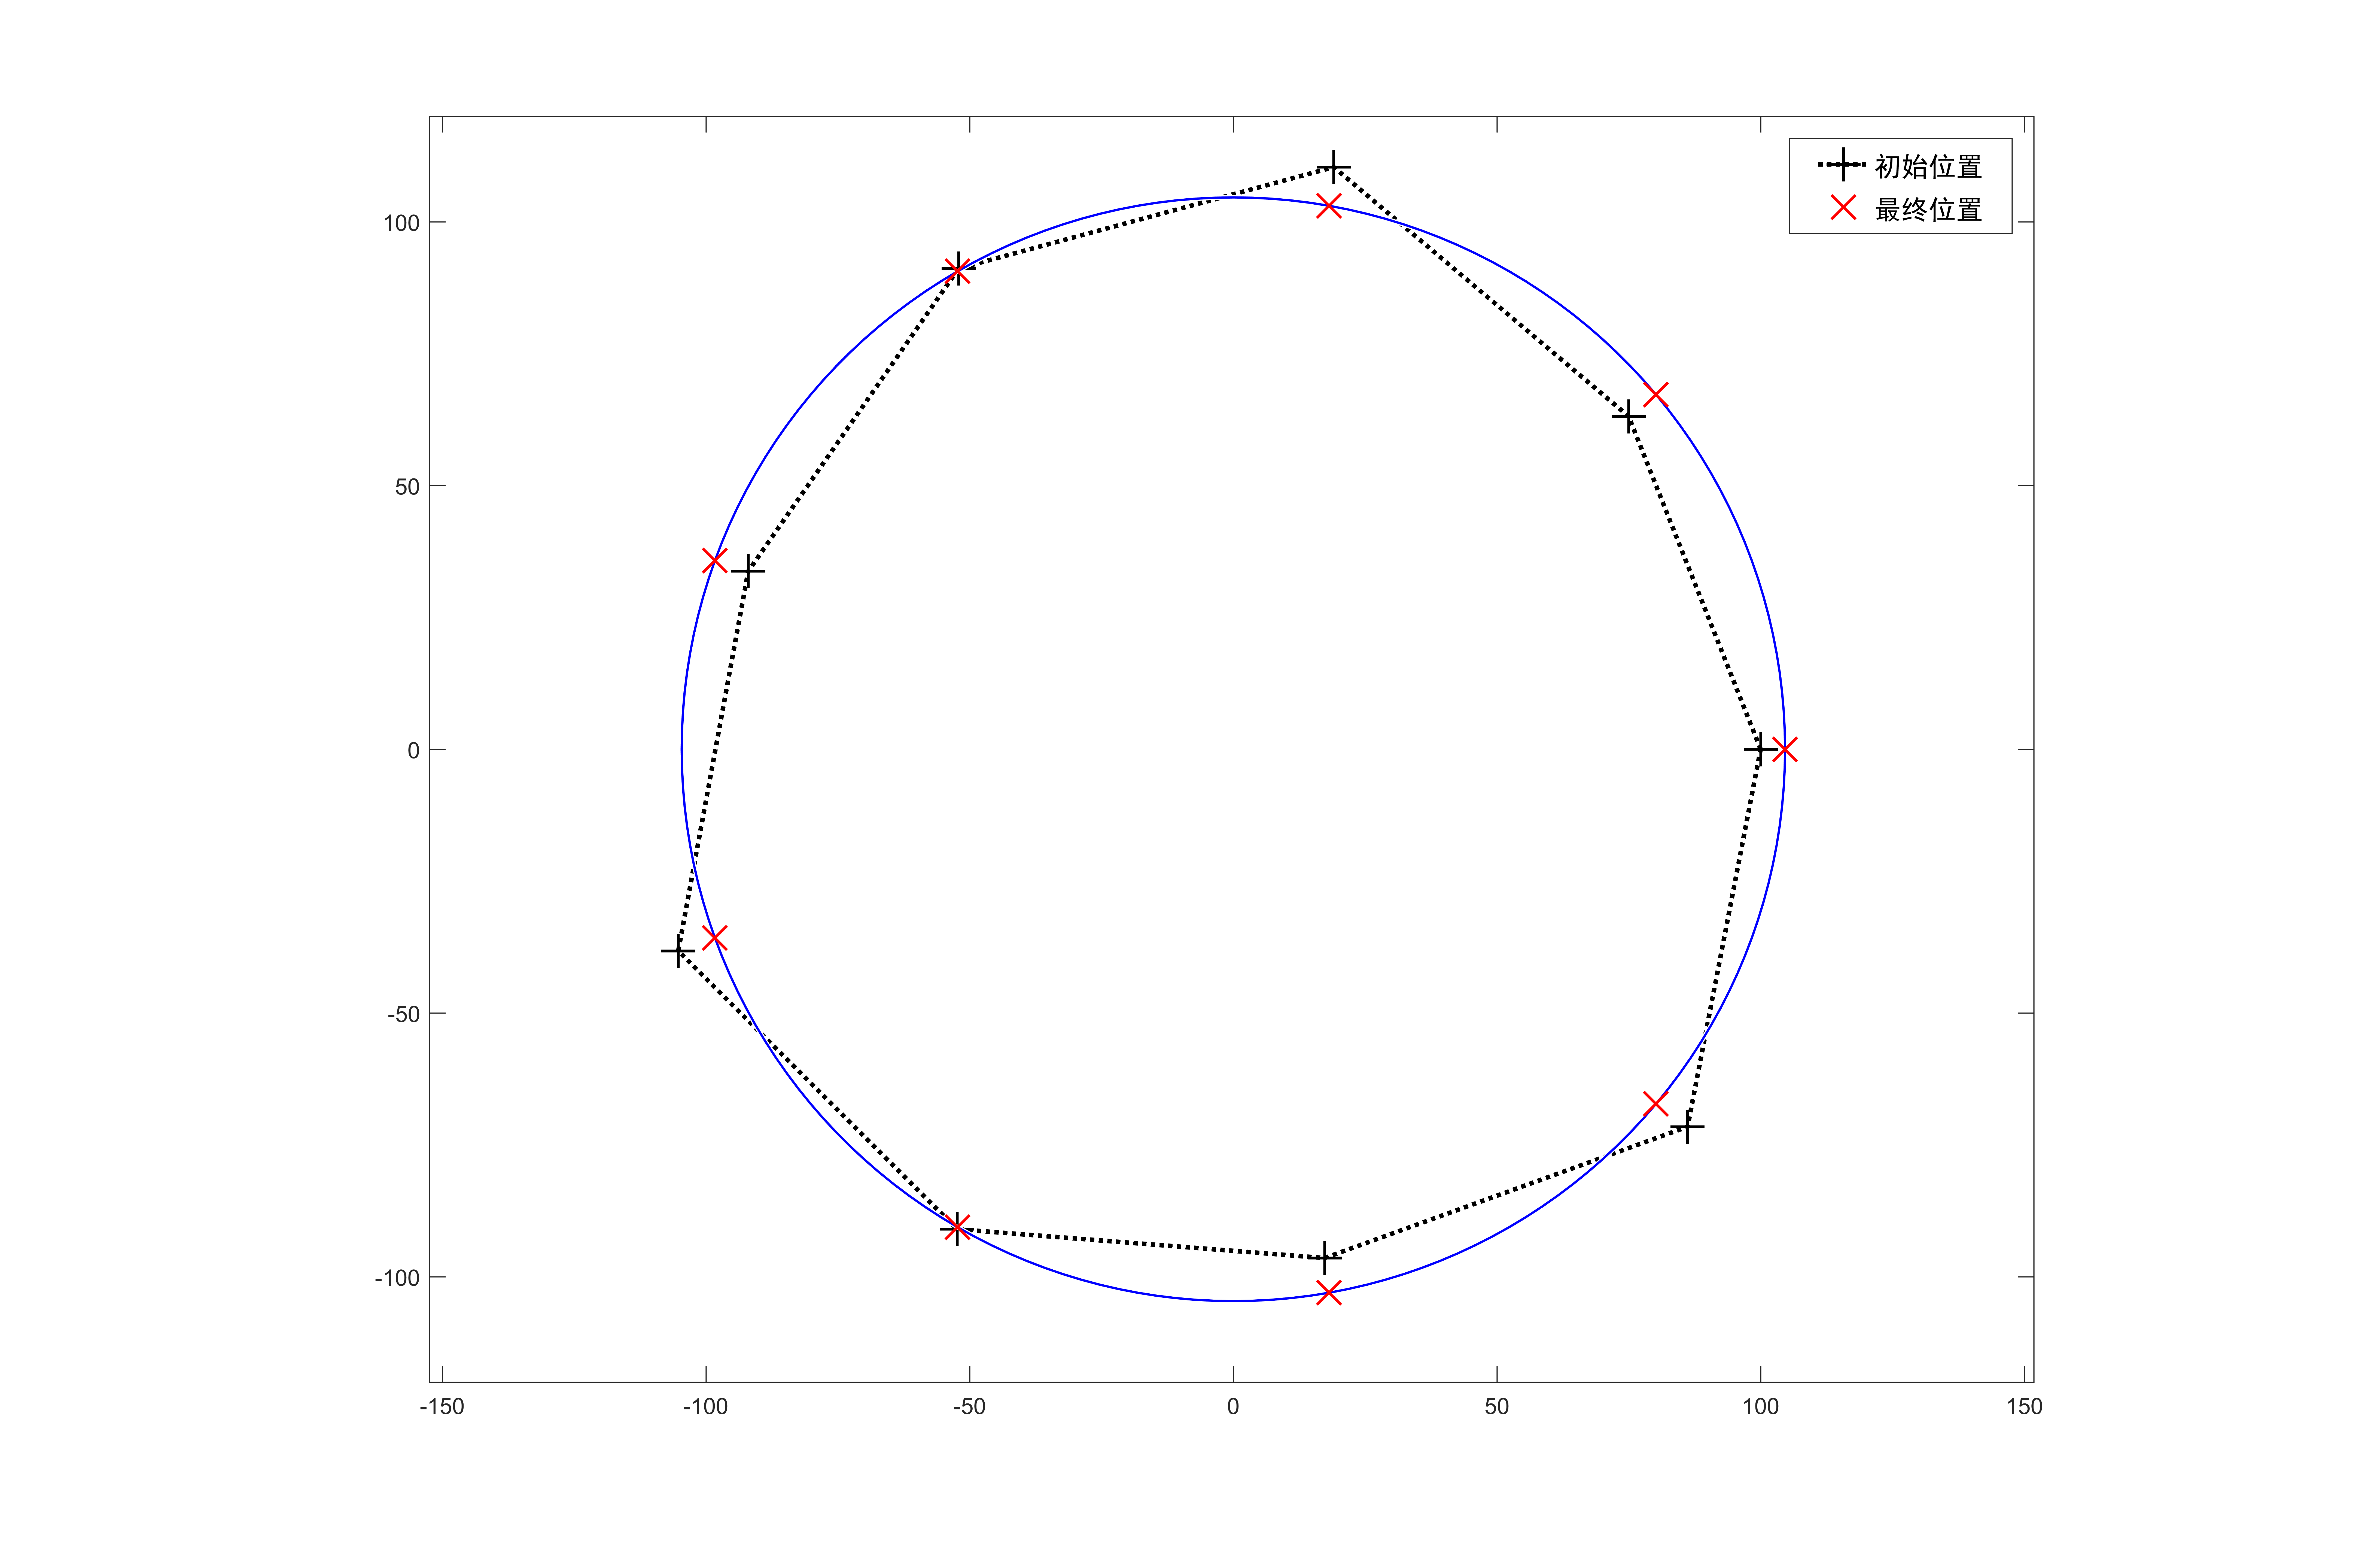
\includegraphics[width=.6\textwidth]{p7}
%	\caption{无人机调整前后位置图}
%	\label{fig:p7}
%\end{figure}

如\cref{fig:p-8}所示,此模型对于无人机位置的调整效果好,且进行九轮位置调整便满足误差<1e-6,进行五轮位置调整后误差<0.01。
%\begin{figure}[H]
%	\centering
%	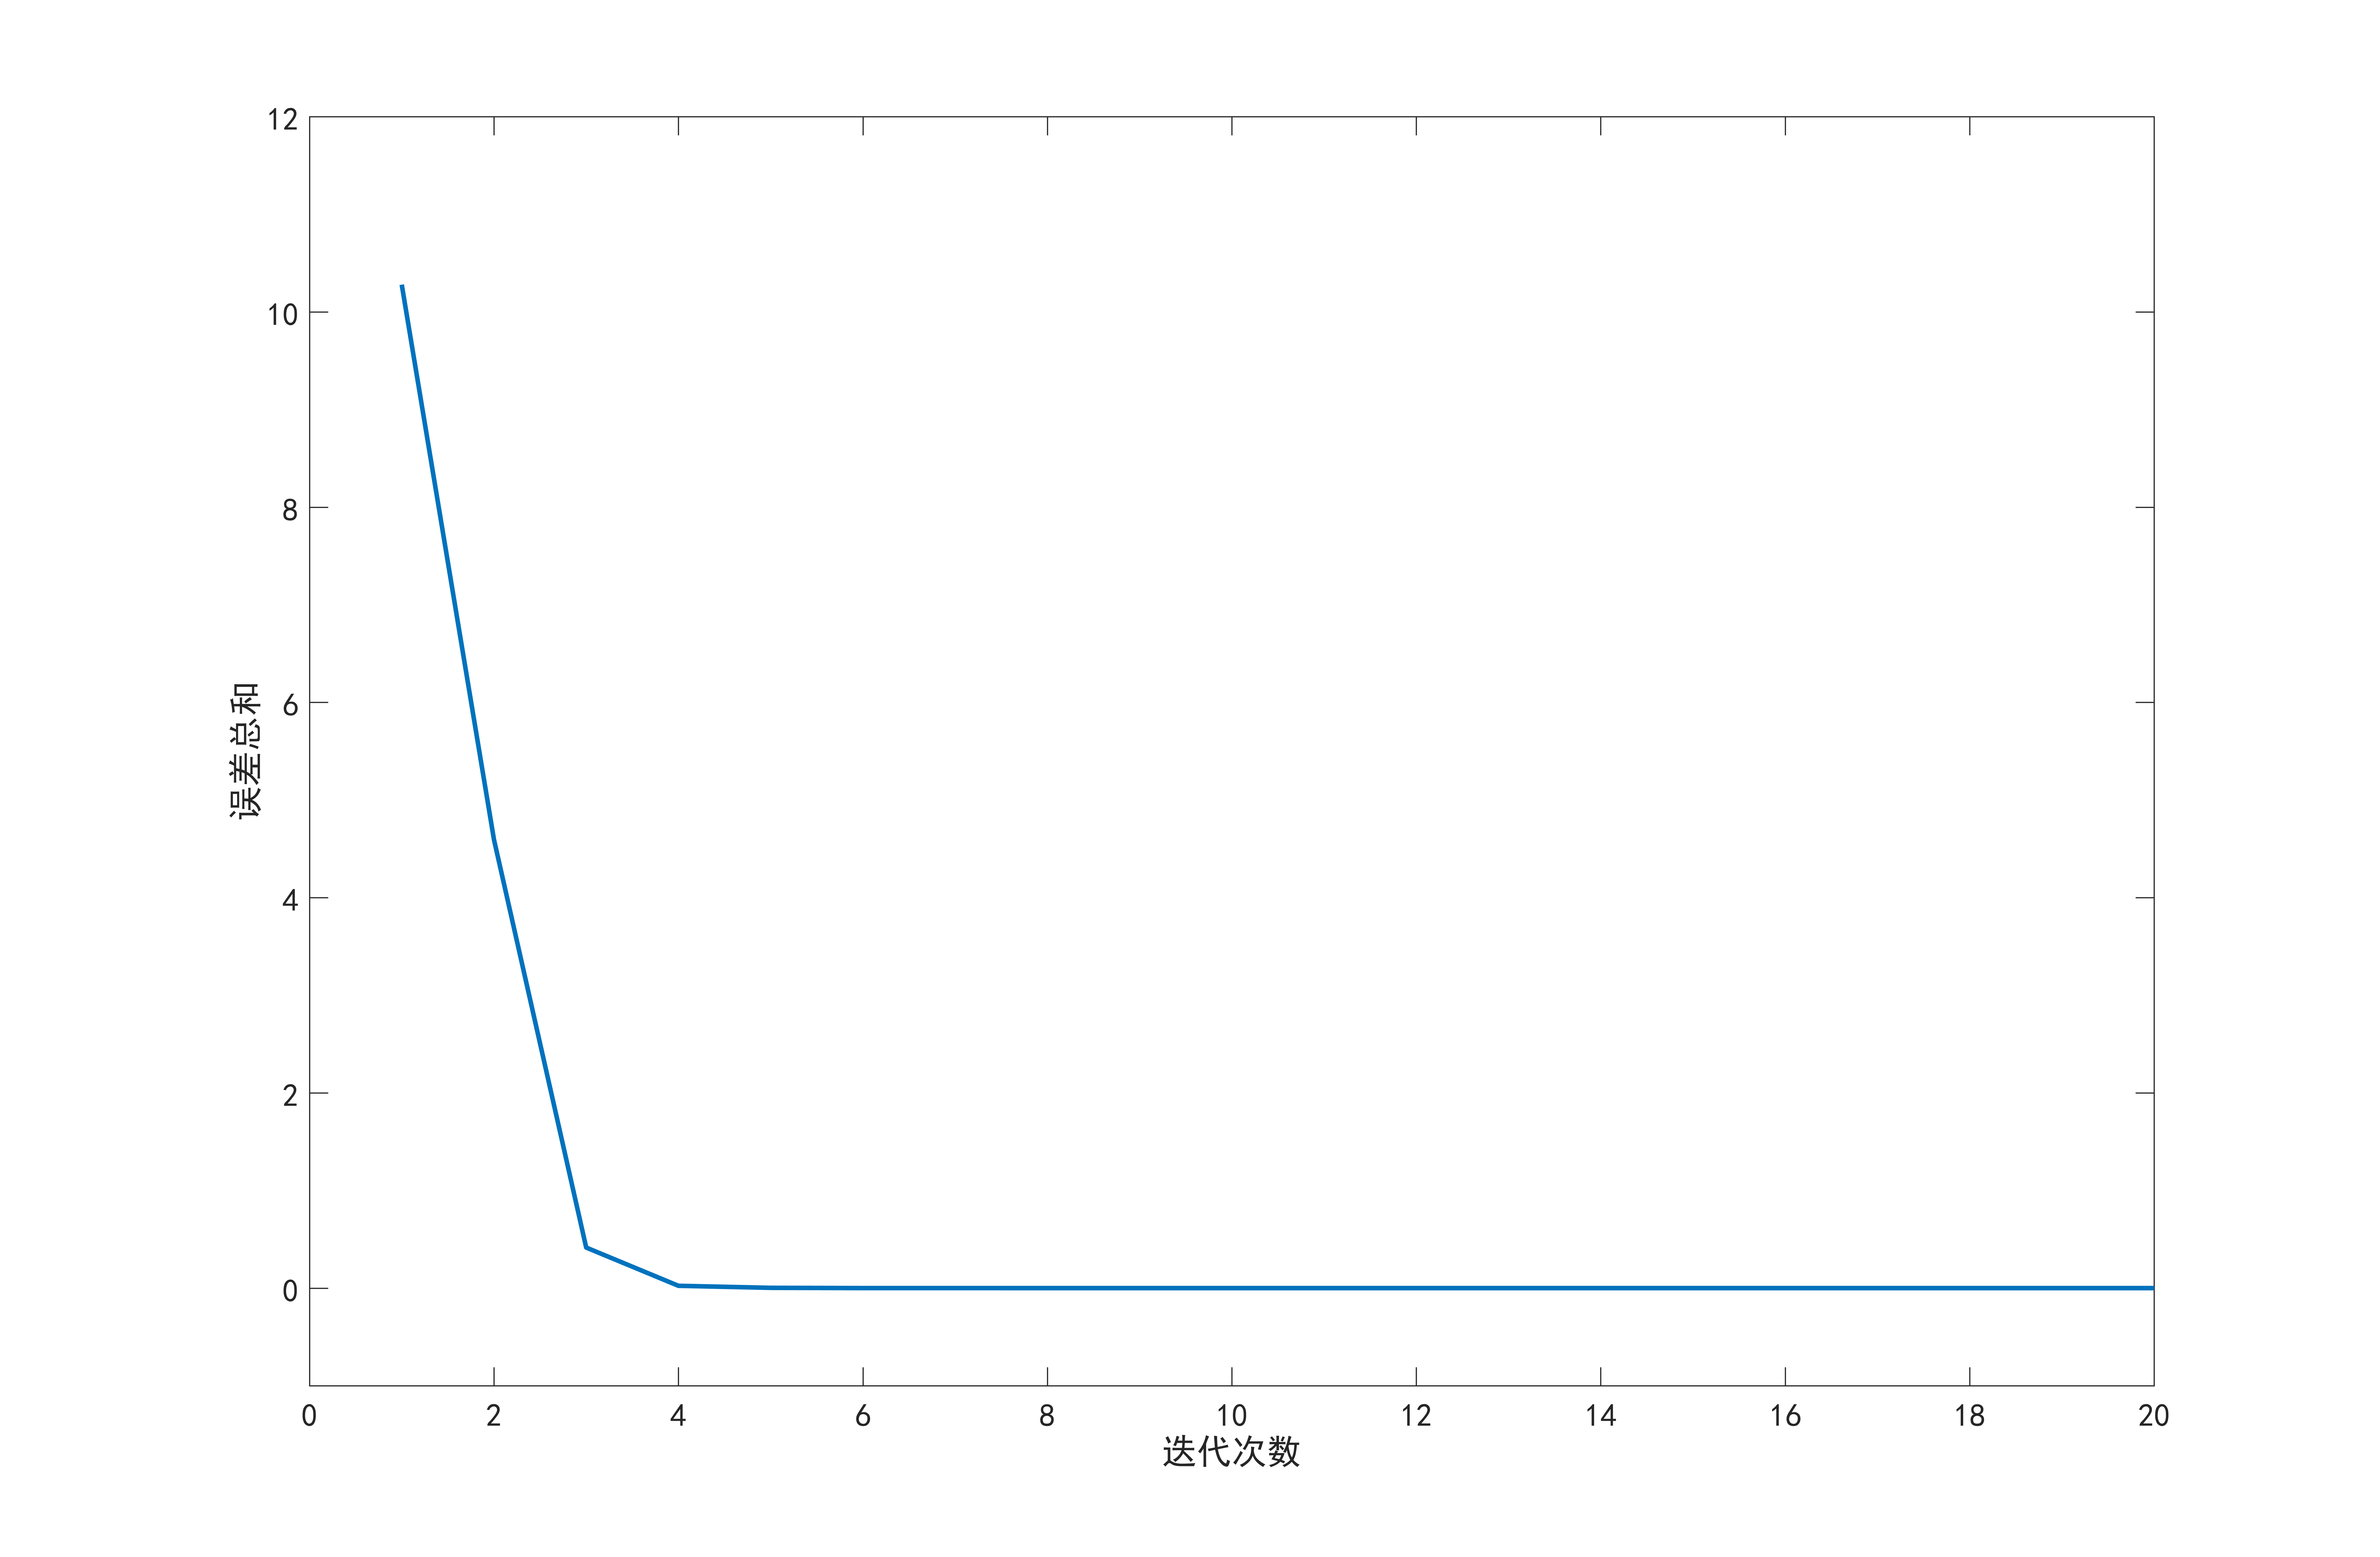
\includegraphics[width=.6\textwidth]{p8}
%	\caption{总误差随迭代次数的变化图}
%	\label{fig:p8}
%\end{figure}
\begin{figure}
	\centering
	\begin{minipage}[c]{0.48\textwidth}
		\centering
		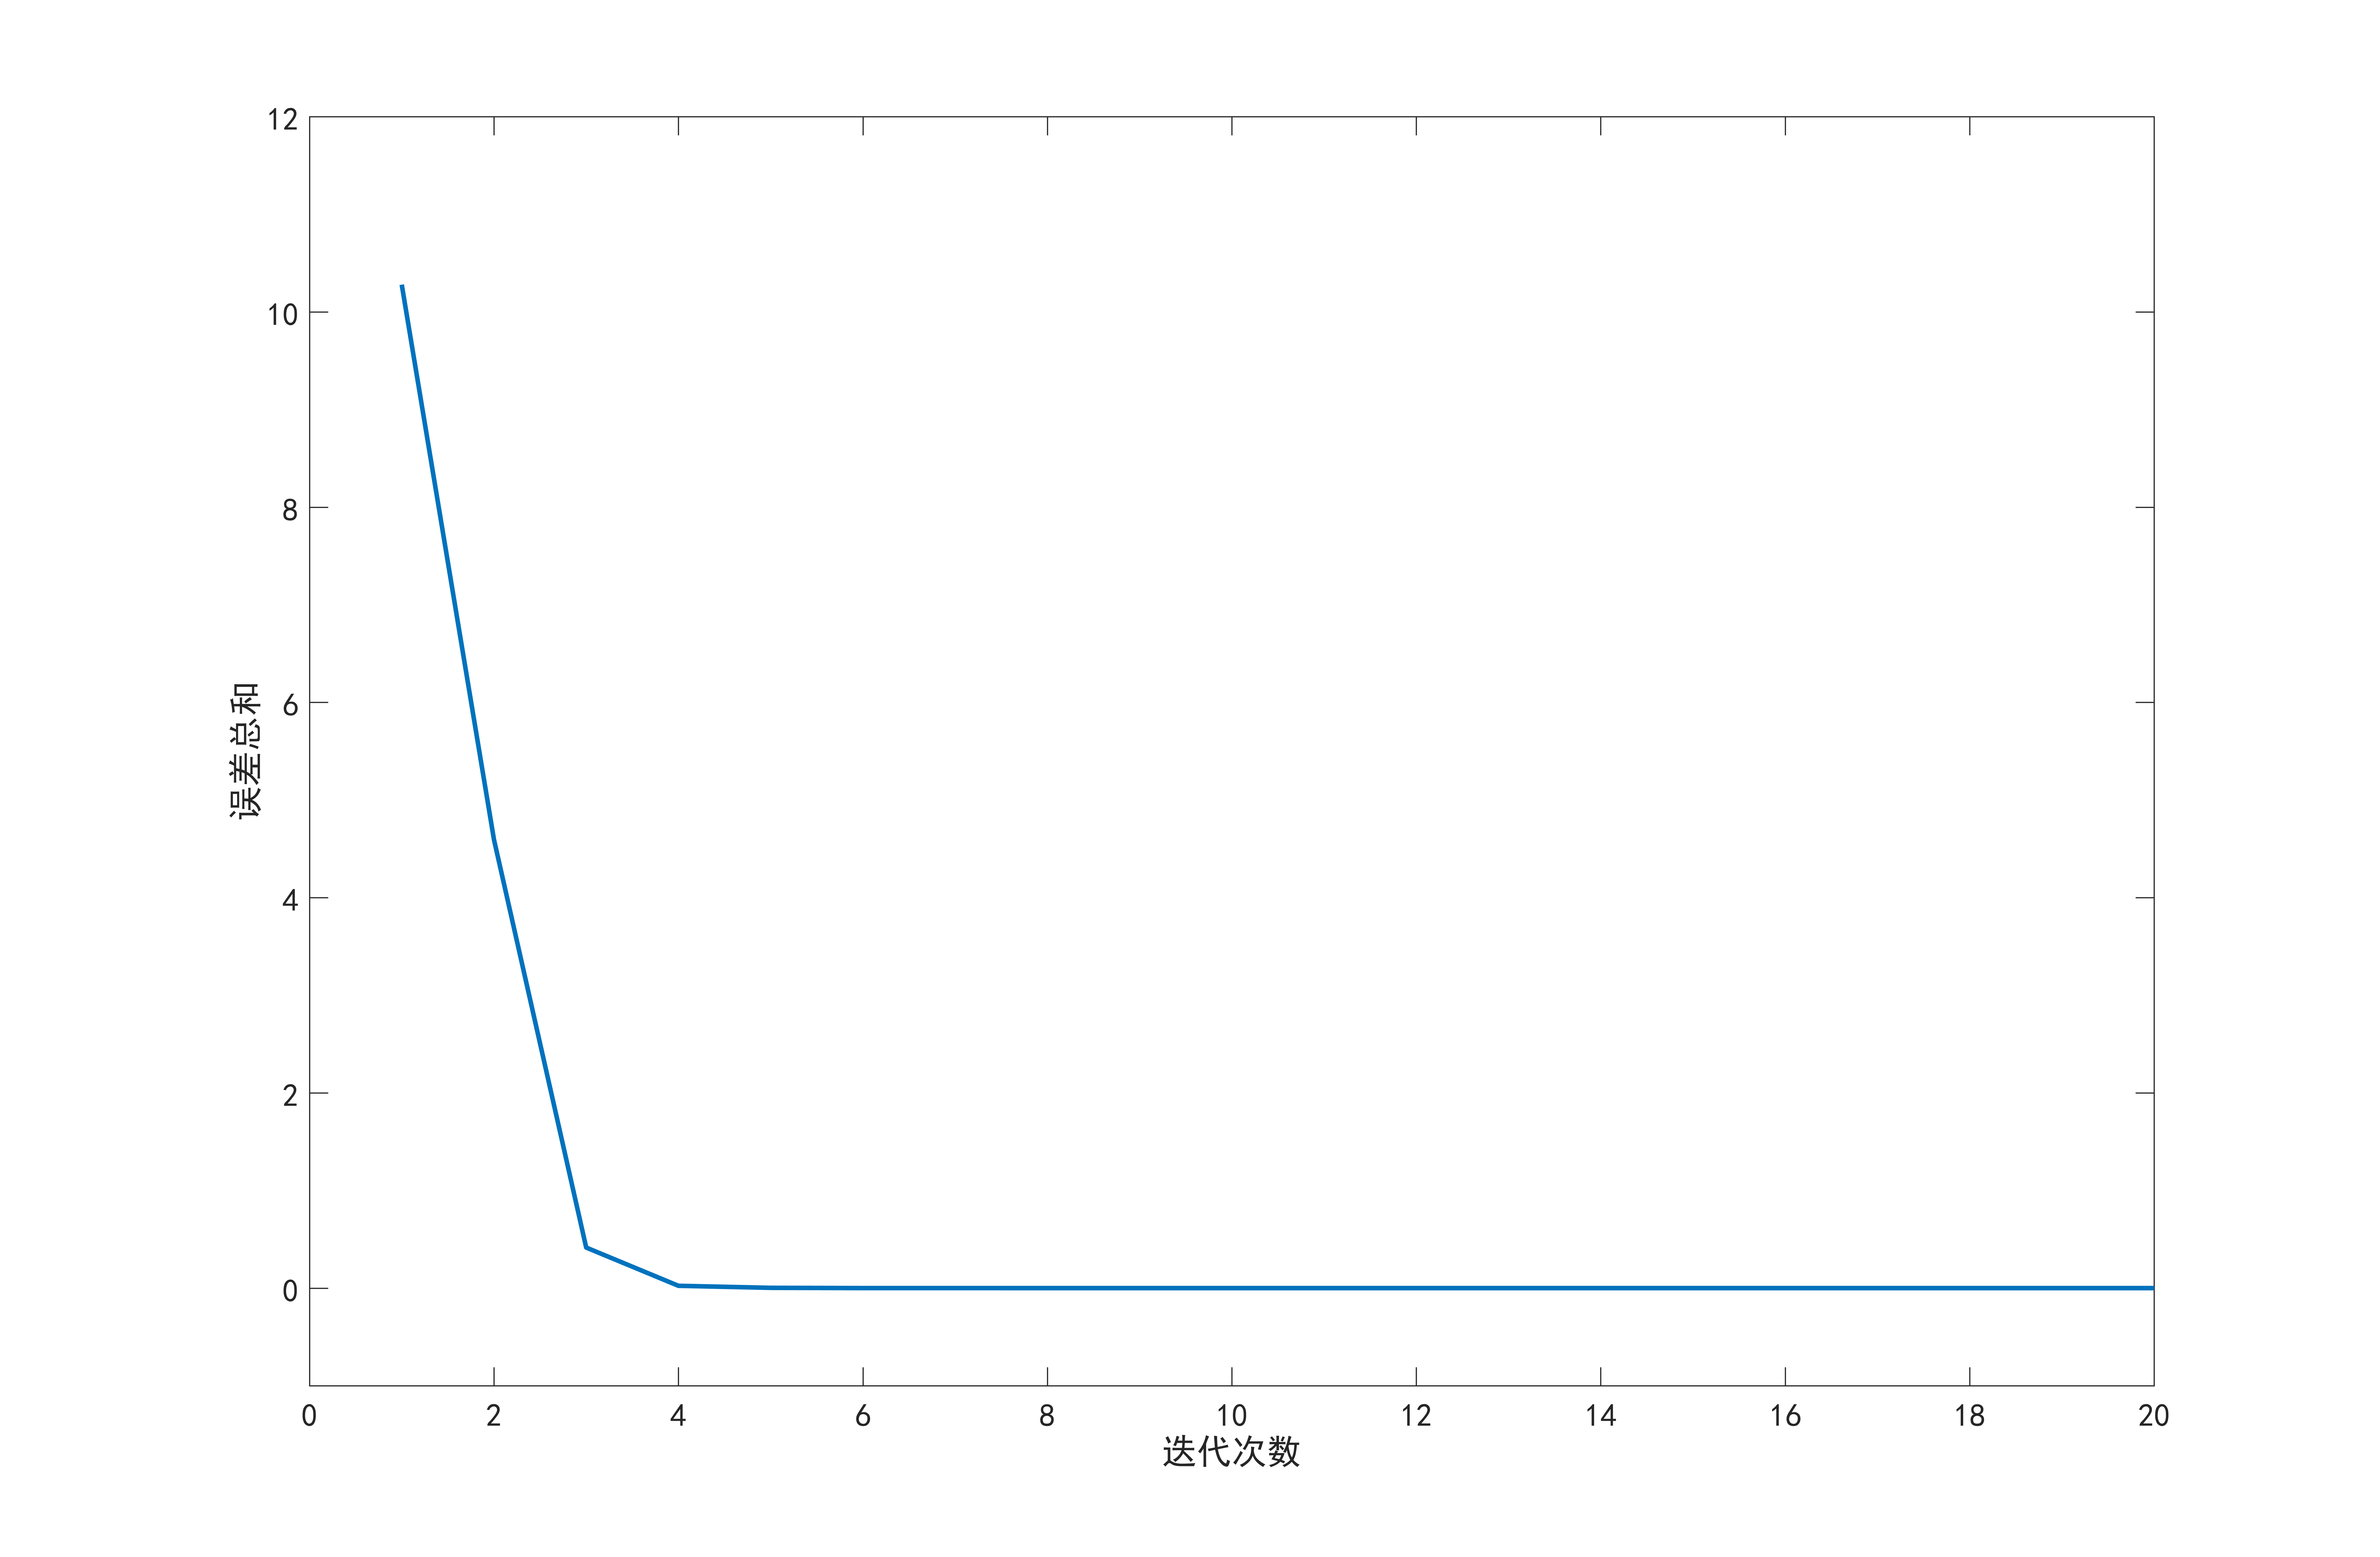
\includegraphics[width=.75\textwidth]{p8}
		\subcaption{总误差随迭代次数的变化图}
		\label{fig:p-8}
	\end{minipage}
	\begin{minipage}[c]{0.48\textwidth}
		\centering
		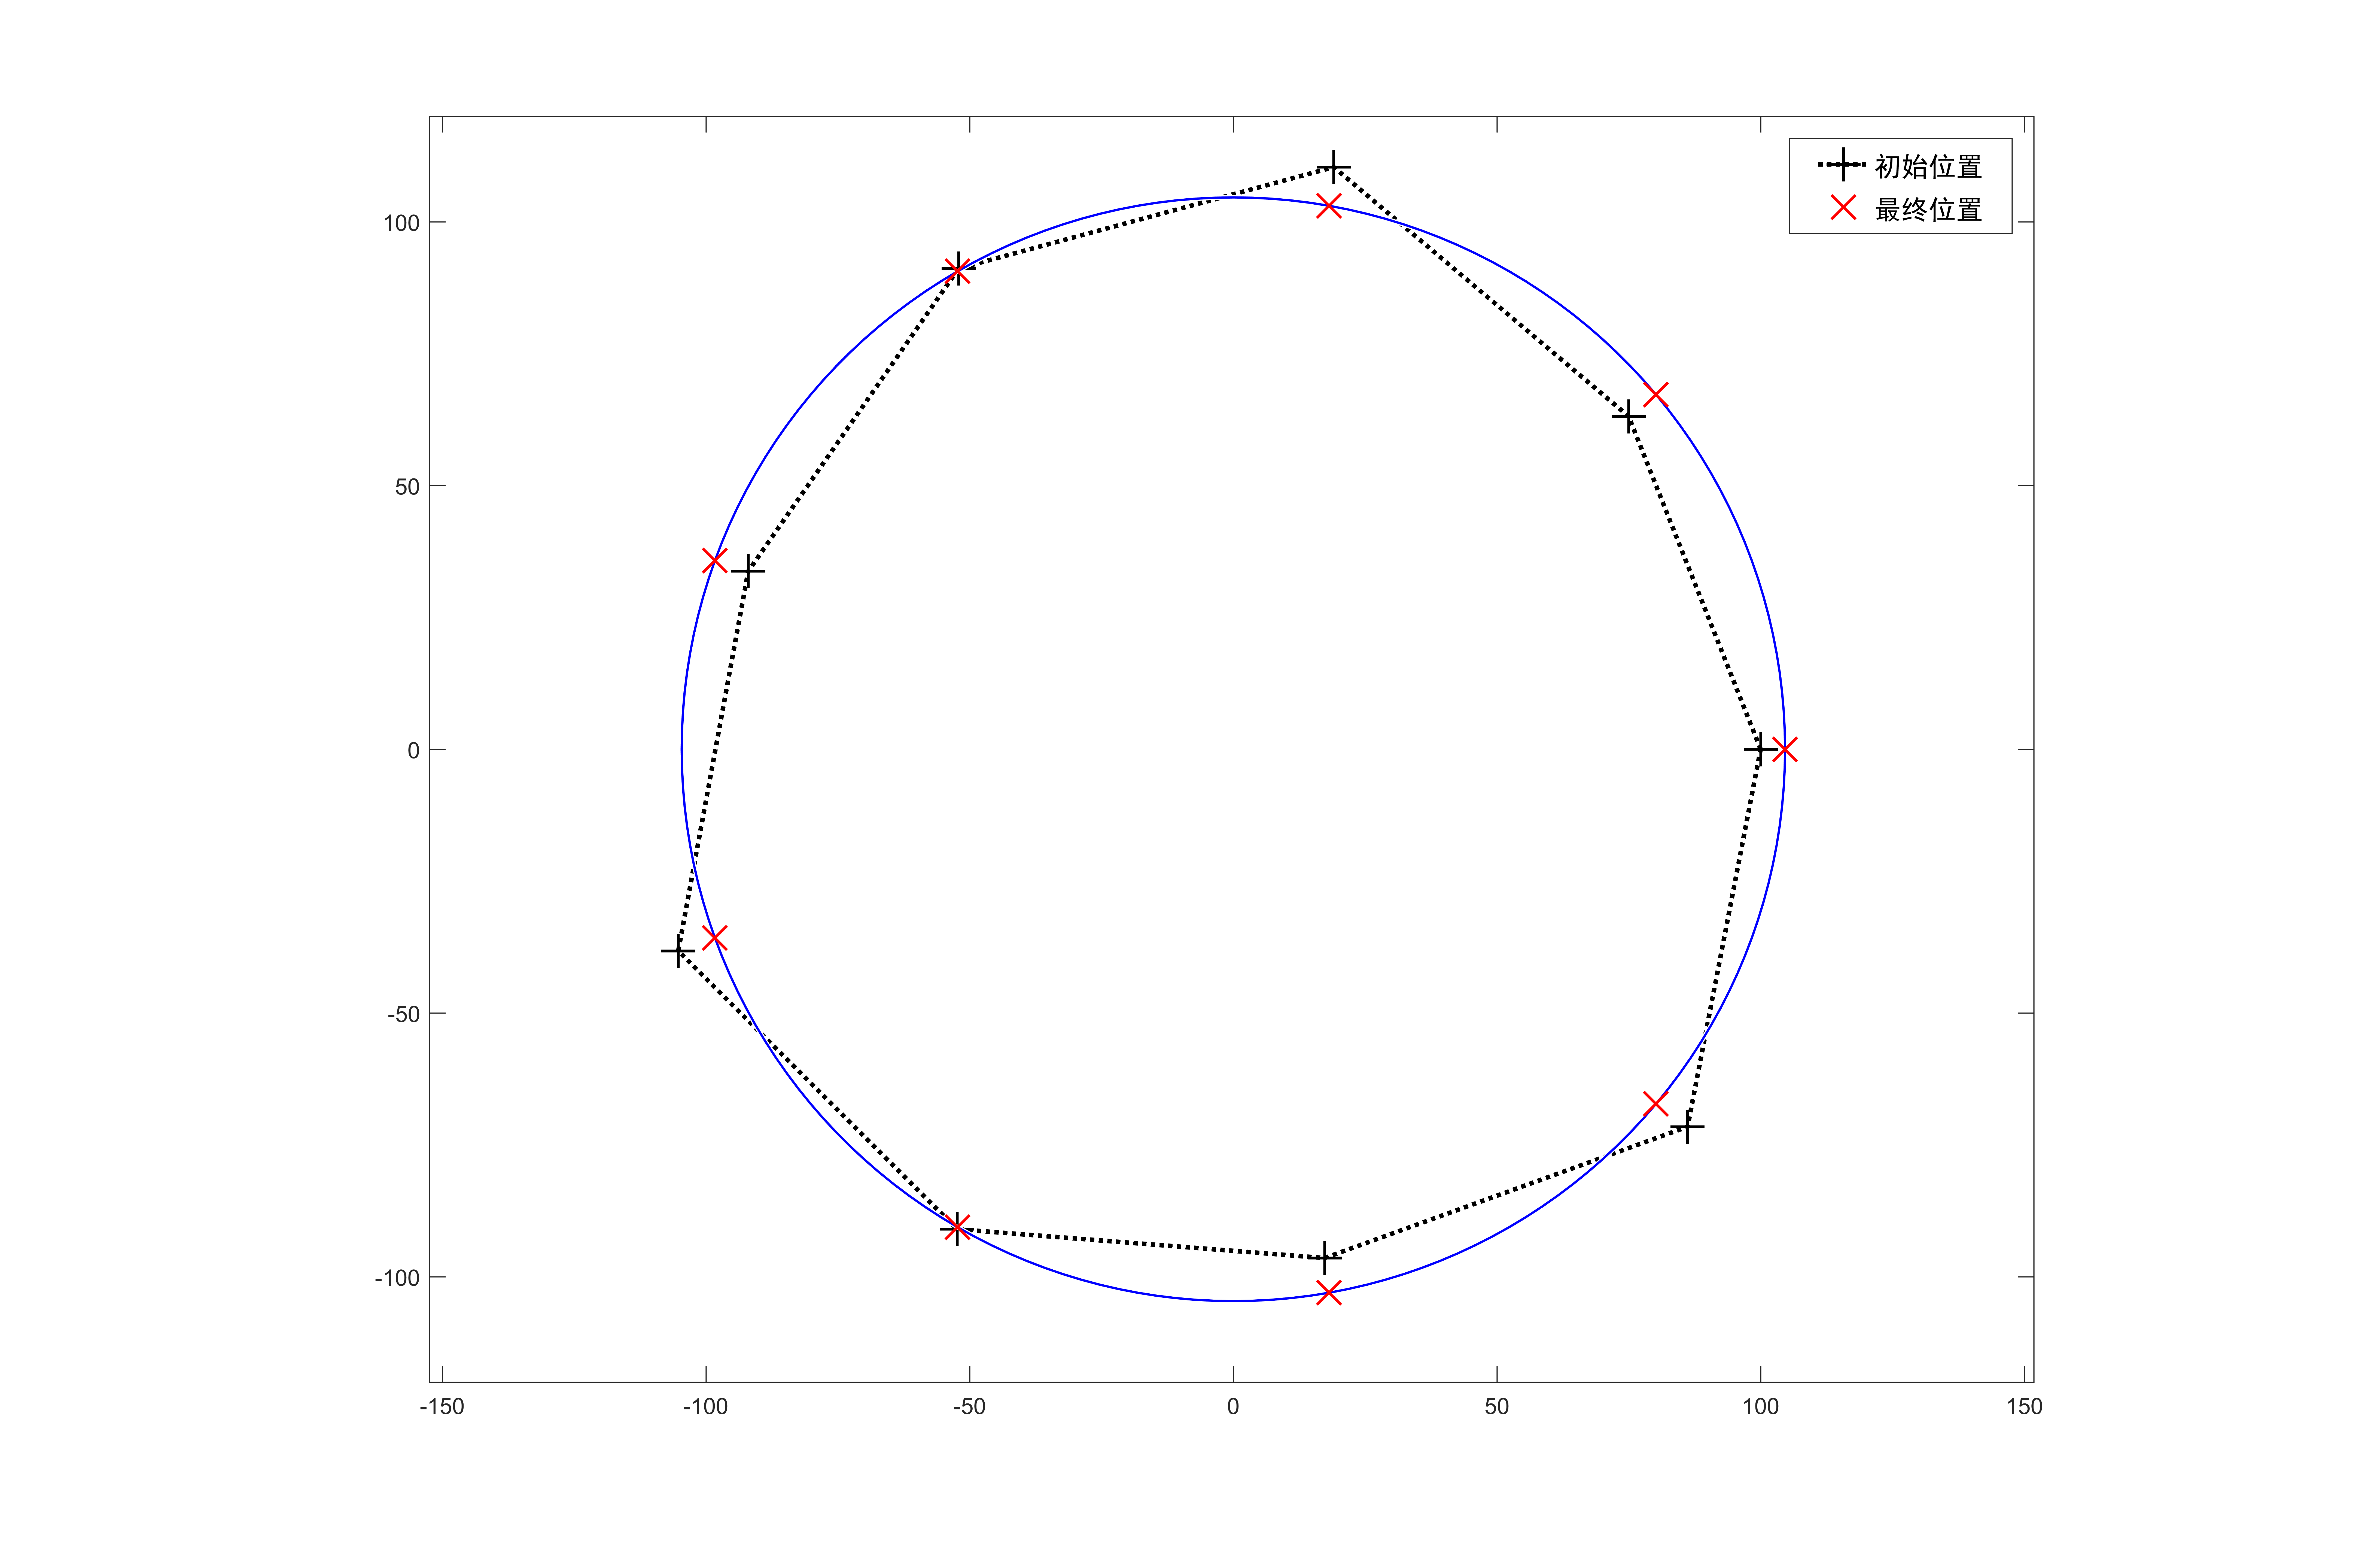
\includegraphics[width=.8\textwidth]{p7}
		\subcaption{无人机调整前后位置图}
		\label{fig:p-7}
	\end{minipage}

	\caption{模型求解结果}
\end{figure}



	

\subsection{问题二的模型建立与求解}
实际生活中,无人机编队可能是圆形、锥形、方形等很多形状。这里我们通过研究锥形来推广第一题所得到的的结论,锥形编队如\cref{fig:p9}所示。为了研究时更能直观的表现出无人机编队形状的特点,我们均假设同一编队的无人机飞行时均位于同一高度上。
\begin{figure}[H]
	\centering
	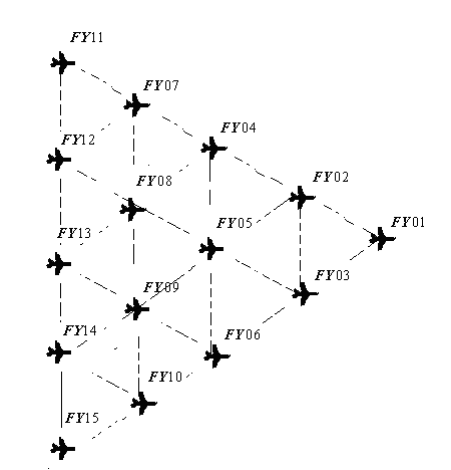
\includegraphics[width=.3\textwidth]{p9}
	\caption{锥形无人机编队示意图}
	\label{fig:p9}
\end{figure}
\subsubsection{确定发射信号无人机数量}
为了便于后续对无人机机定位,我们取编号为FY13的飞机作为参照飞机,即FY13的坐标为$(0,0)$。同时,定义标准情况FY13-FY01的方向为x轴正方向,建立直角坐标系。下面对除了无人机FY13以外还需要几架飞机进行讨论:

1. 只增加一架无人机。此时由于信号发射机与任意一架接收机一共只有三个无人机。由于三个点仅能确定一个圆,也即信号接收机的可能轨迹是一个圆。此时无法实现对信号接收机的准确定位。故这种情况不存在
 
2. 增加两架无人机。此时信号发射机与信号接收机一共四架无人机。由于过三点可以确定一个圆,所以过未知无人机$M'$的圆一共有三个,也即这三个圆的交点即为待接收信号无人机的位置。又根据三个互相相交圆的交点个数可能为一个或两个,所以这里进行进一步讨论:
\begin{figure}[H]
	\centering
	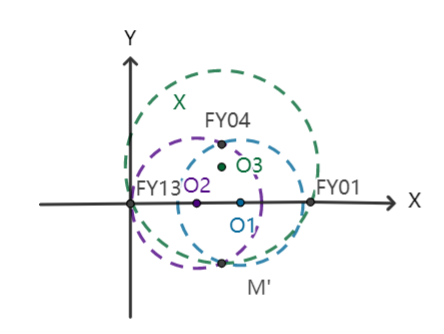
\includegraphics[width=.55\textwidth]{p10}
	\caption{锥形无人机定位图}
	\label{fig:p10}
\end{figure}
(1) 发射信号的两架无人机坐标相较于FY13均标准,也即发射信号的无人机所处位置均无偏差。
如\cref{fig:p10}所示,取无人机$FY01(2\sqrt{3} \rho,0)$与$FY04(\sqrt{3} \rho,\sqrt{3} \rho)$发射信号,其中$\rho$为相邻两架飞机之间距离的长度。取点$FY04,FY01,M'$构成$\odot O_1$,点$FY04,FY13,M'$构成$\odot O_2$,点$FY01,FY13,M'$构成$\odot O_3$,根据公式\cref{eq:14},其方程组分别为:
\[
%\begin{equation}
\begin{cases}
	(x_1-\sqrt{3}\rho)^2+(y_1-\rho)^2=r_3^2\\
	(x_1-2\sqrt{3}\rho)^2+y_1^2=r_1^2\\
	\rho=r_1\sin \alpha_1
\end{cases}
%\end{equation}
\]
\[
%\begin{equation}
\begin{cases}
	x_2^2+y_2^2=r_1^2\\
	(x_2-\sqrt{3}\rho)^2+(y_2-\rho)^2=r_2^2\\
	\rho=r_2\sin \alpha_2
\end{cases}
%\end{equation}
\]
\[
%\begin{equation}
\begin{cases}
x_3^2+y_3^2=r_3^2\\
(x_3-2\sqrt{3}\rho)^2+y_3^2=r_3^2\\
\sqrt{3}\rho=r_3\sin \alpha_3
\end{cases}
%\end{equation}
\]

解得:
\begin{equation}
	\begin{cases}
		r_1=\frac{\rho}{\sin \alpha_1}\\
		x_1=\frac{3\sqrt{3} \rho +  \cot \alpha_1}{2}\\
		y_1=\sqrt{3}x_1-4\rho
	\end{cases}
	\label{eq:28}
\end{equation}
\begin{equation}
	\begin{cases}
		r_2=\frac{\rho}{\sin \alpha_2}\\
		x_2=\frac{\sqrt{3} \rho + \rho \cot \alpha_2}{2}\\
		y_2=2\rho-\sqrt{3}x_2
	\end{cases}
	\label{eq:29}
\end{equation}
\begin{equation}
	\begin{cases}
		r_3=\frac{\sqrt{3}\rho}{\sin^2 \alpha_3}\\
		x_3=\sqrt{3} \rho \\
		y_3=\sqrt{3} \rho \cot^2 \alpha
	\end{cases}
	\label{eq:30}
\end{equation}

综上,式\cref{eq:14}\cref{eq:28}\cref{eq:29}\cref{eq:30}$(i \ne 4)$为对于无人机$M'$的定位模型

与问题一第(2)问类似,根据式\cref{eq:20}\cref{eq:21}采用最小二乘法进行求解验证,此情况成立,即三架无人机发射信号即可对剩余无人机完成有效定位

(2)如果除FY13以外的所有无人机坐标可能存在误差的情况,上述方程将会新增两个未知数故无法求解,所以我们考虑再增加一架信号发射无人机进行求解。



\subsubsection{锥形编队无人机定位调度模型}
在圆形编队中,无人机的实际点与计算点具有较为特殊的性质,其主要原因是圆的对称性强且圆上点到圆心的距离是相同的。在本编队中,我们的原点取得是FY13这一架飞机所在位置,显然在本编队中,各飞机到达原点位置是不同的,因此无人机无法再认为所接受到的角是从发射机的原编队位置发射来的。但是无人机可以寻找一个点使得认为从发射机原编队位置发射信号所形成角度尽可能地接近原始接收到的角度,基于以上思想,我们提出一种基于最小化接受角误差的无人机定位模型。具体描述如下:
\begin{figure}[H]
	\centering
	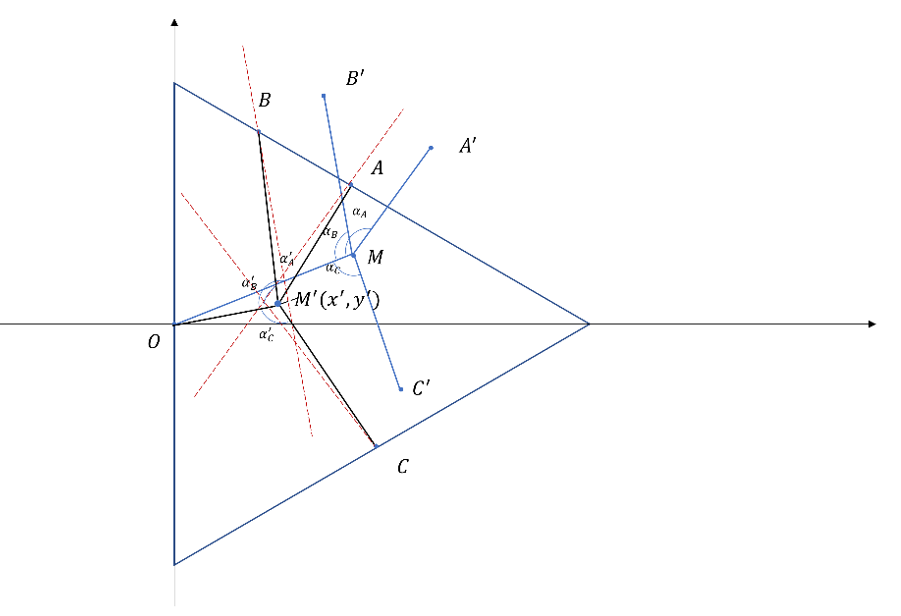
\includegraphics[width=.55\textwidth]{p11}
	\caption{锥形无人机定位图}
	\label{fig:p11}
\end{figure}
首先过$A$作$A^\prime M$的平行线$l_A$,过$B$做$B^\prime M$的平行线$l_B$,过$C$做$C^\prime M$的平行线$l_C$,由于锥形编队的特点,显然三条直线不存在唯一的交点,而是围成一个三角形区域。此时期望从中找一点$M^\prime$使得分别所接收到的角与$M$处接收到的角尽可能接近,如\cref{fig:p11}所示。由于该角属于$[0,\pi]$中,因此使用余弦进行衡量,目标函数如下:
\begin{equation}
		\min \sum_{i=1}^{n}{|cos\alpha_i^\prime-cos\alpha_i|}
	\label{eq:31}
\end{equation}
设点$M^\prime=(x^\prime,y^\prime)$,则有
\begin{equation}
	\cos \alpha_i^\prime=\frac{\vec{M^\prime\ O}\ \cdot\vec{M^\prime B}}{\vec{{|M}^\prime O}|\ \cdot\vec{{|M}^\prime B}|}=\frac{{x^\prime}^2+{y^\prime}^2-x^\prime x_i-y^\prime y_i}{{{2x}^\prime}^2+{{2y}^\prime}^2-{2x}^\prime x_i-{2y}^\prime y_i+x_i^2+y_i^2}
	\label{eq:32}
\end{equation}
假设$l_A$、$l_B$、$l_C$直线方程分别为:
\begin{equation}
	l_A:\ A_1x+B_1y+C_1=0 //
	l_B:\ A_2x+B_2y+C_2=0//
	l_C:\ A_3x+B_3y+C_3=0
	\label{eq:33}
\end{equation}
由$A^\prime M$直线与$B^\prime M$和$C^\prime M$能够求得上述式子中的$A$和$B$,其中$C$通过$M^\prime$点进行求解。具体过程略。

因此,该处的目标为在三条之间所夹的区域内确定$M^\prime=(x^\prime,y^\prime)$使得目标函数最小。约束条件如下:
\begin{equation}
	{(A}_1x^\prime+B_1y^\prime+C_1)\ast{(A}_2x^\prime+B_2y^\prime+C_2)\ast{(A}_3x^\prime+B_3y^\prime+C_3)\le0
	\label{eq:34}
\end{equation}

使用matlab对上述式子进行求解,解得结果即为M点的计算位置$M^\prime$。

其余调度思想与问题一第(3)问相同。
\subsubsection{模型求解}

首先确定锥形无人机的初始位置(有误差)。根据无人机锥形编队的性质:直线上相邻两架无人机的间距相等为 50 m,可以在直角坐标系下计算出无人机的标准位置。基于标准位置设置10\%的误差,计算得到有误差的初始位置,见附录\cref{tab:4}

具体求解思想与问题一第(3)问相同,采用贪心算法。

初始条件下的模拟结果如\cref{tab:a}所示,选出第一轮总误差最小的发射信号无人机方案:FY01,FY09,FY10
\begin{table}[!htbp]
	\caption{第一轮模拟结果}\label{tab:a} \centering
	\begin{tabular}{cccccc}
		\toprule[1.5pt]
		模拟次数 & 无人机方案 & FY01误差 & $\cdots$ & FY15误差 & 总误差\\
		\midrule[1pt]
		1 & FY01,FY02,FY04 & 1.11485 & 	$\cdots$ & 12.0180 & 2985.47\\
		2 & FY01,FY02,FY05 & 1.11485 & 	$\cdots$ &12.0180&2984.57 \\
		3 & FY01,FY02,FY06 & 1.11485 & 	$\cdots$ &12.0180&2983.45\\
		$\cdots$ & $\cdots$ & $\cdots$ & $\cdots$ & $\cdots$ & $\cdots$\\
		352 & FY12,FY14,FY15 & 29.5770 & 	$\cdots$ & 4.50855& 169.547\\
		\bottomrule[1.5pt]
	\end{tabular}
\end{table}

通过matlab模拟多轮进行求解,得到发射信号无人机的选择方案如\cref{tab:b}所示。
	
\begin{table}[H]
	\caption{发射信号无人机的选择方案}\label{tab:b} \centering
	\begin{tabular}{ccccc}
		\toprule[1.5pt]
		调整次数 &  & 无人机方案 &  & 总误差 \\
		\midrule[1pt]
		1 & FY01 & FY09 & FY10 & 18.4047
		\\
		2 & FY03 & FY04 & FY05 & 15.3164
		\\
		3 & FY7 & FY12 & FY15 & 12.2350
		\\ 
		%		4 & FY02 & FY05 & FY09 & 0.023668\\
		%		5 & FY01 & FY07 & FY08 & 0.002855\\
		%		6 & FY02 & FY03 & FY09 & 0.000218\\
		%		7 & FY02 & FY05 & FY07 & 0.000056\\
		%		8 & FY03 & FY04 & FY06 & 4.29283E-06\\
		%		9 & FY01 & FY06 & FY07 & 8.61033E-07\\
		$\cdots$ & $\cdots$ & $\cdots$ & $\cdots$ & $\cdots$ \\
		50 & FY03 & FY11 & FY15 & 0.0779
		\\
		\bottomrule[1.5pt]
	\end{tabular}
\end{table}	
那么无人机的调整方案为:根据\cref{tab:b}进行发射信号无人机的选择,其余无人机接收方位信息进行调整,进行迭代,大概十轮误差收敛,无人机调整完毕的位置见附录\cref{tab:5},与初始位置进行对比如\cref{fig:p-11}所示

%\end{figure}
\begin{figure}
	\centering
	\begin{minipage}[c]{0.48\textwidth}
		\centering
		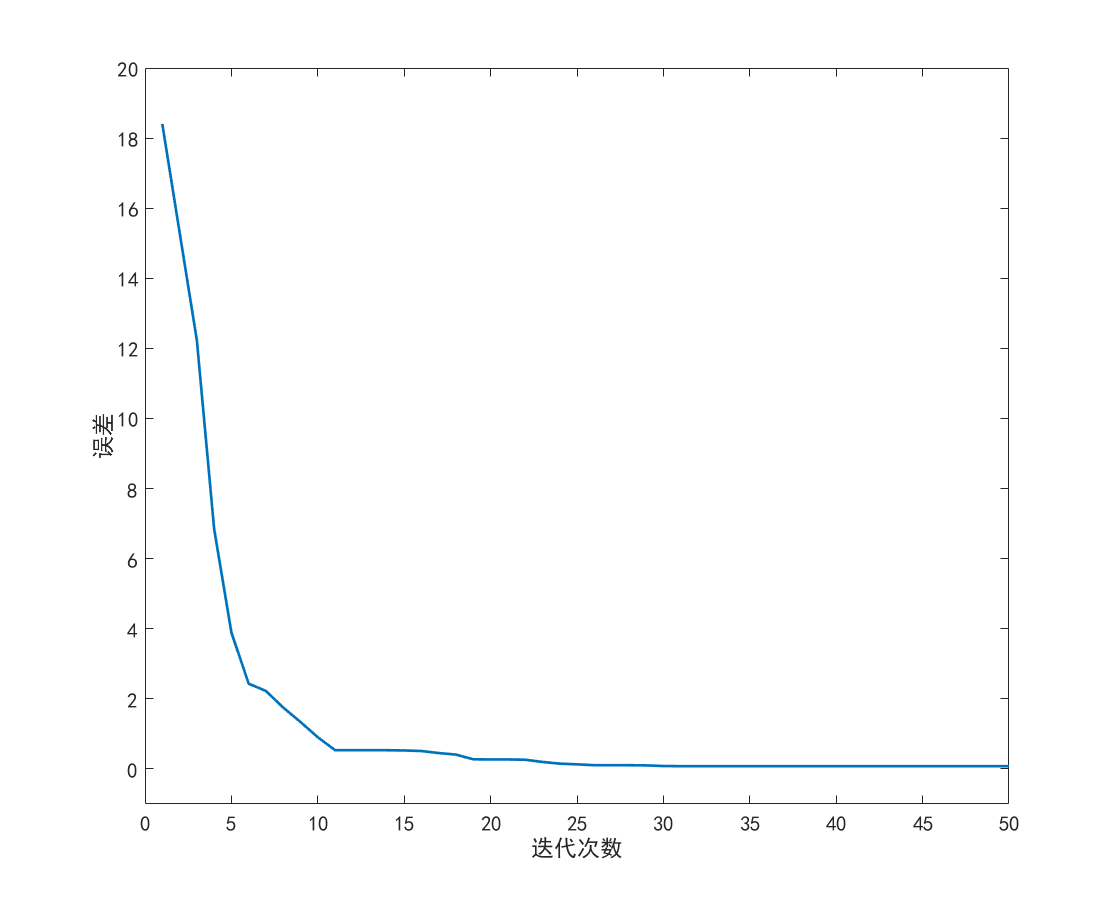
\includegraphics[width=.75\textwidth]{p12}
		\subcaption{总误差随迭代次数的变化图}
		\label{fig:p-11}
	\end{minipage}
	\begin{minipage}[c]{0.48\textwidth}
		\centering
		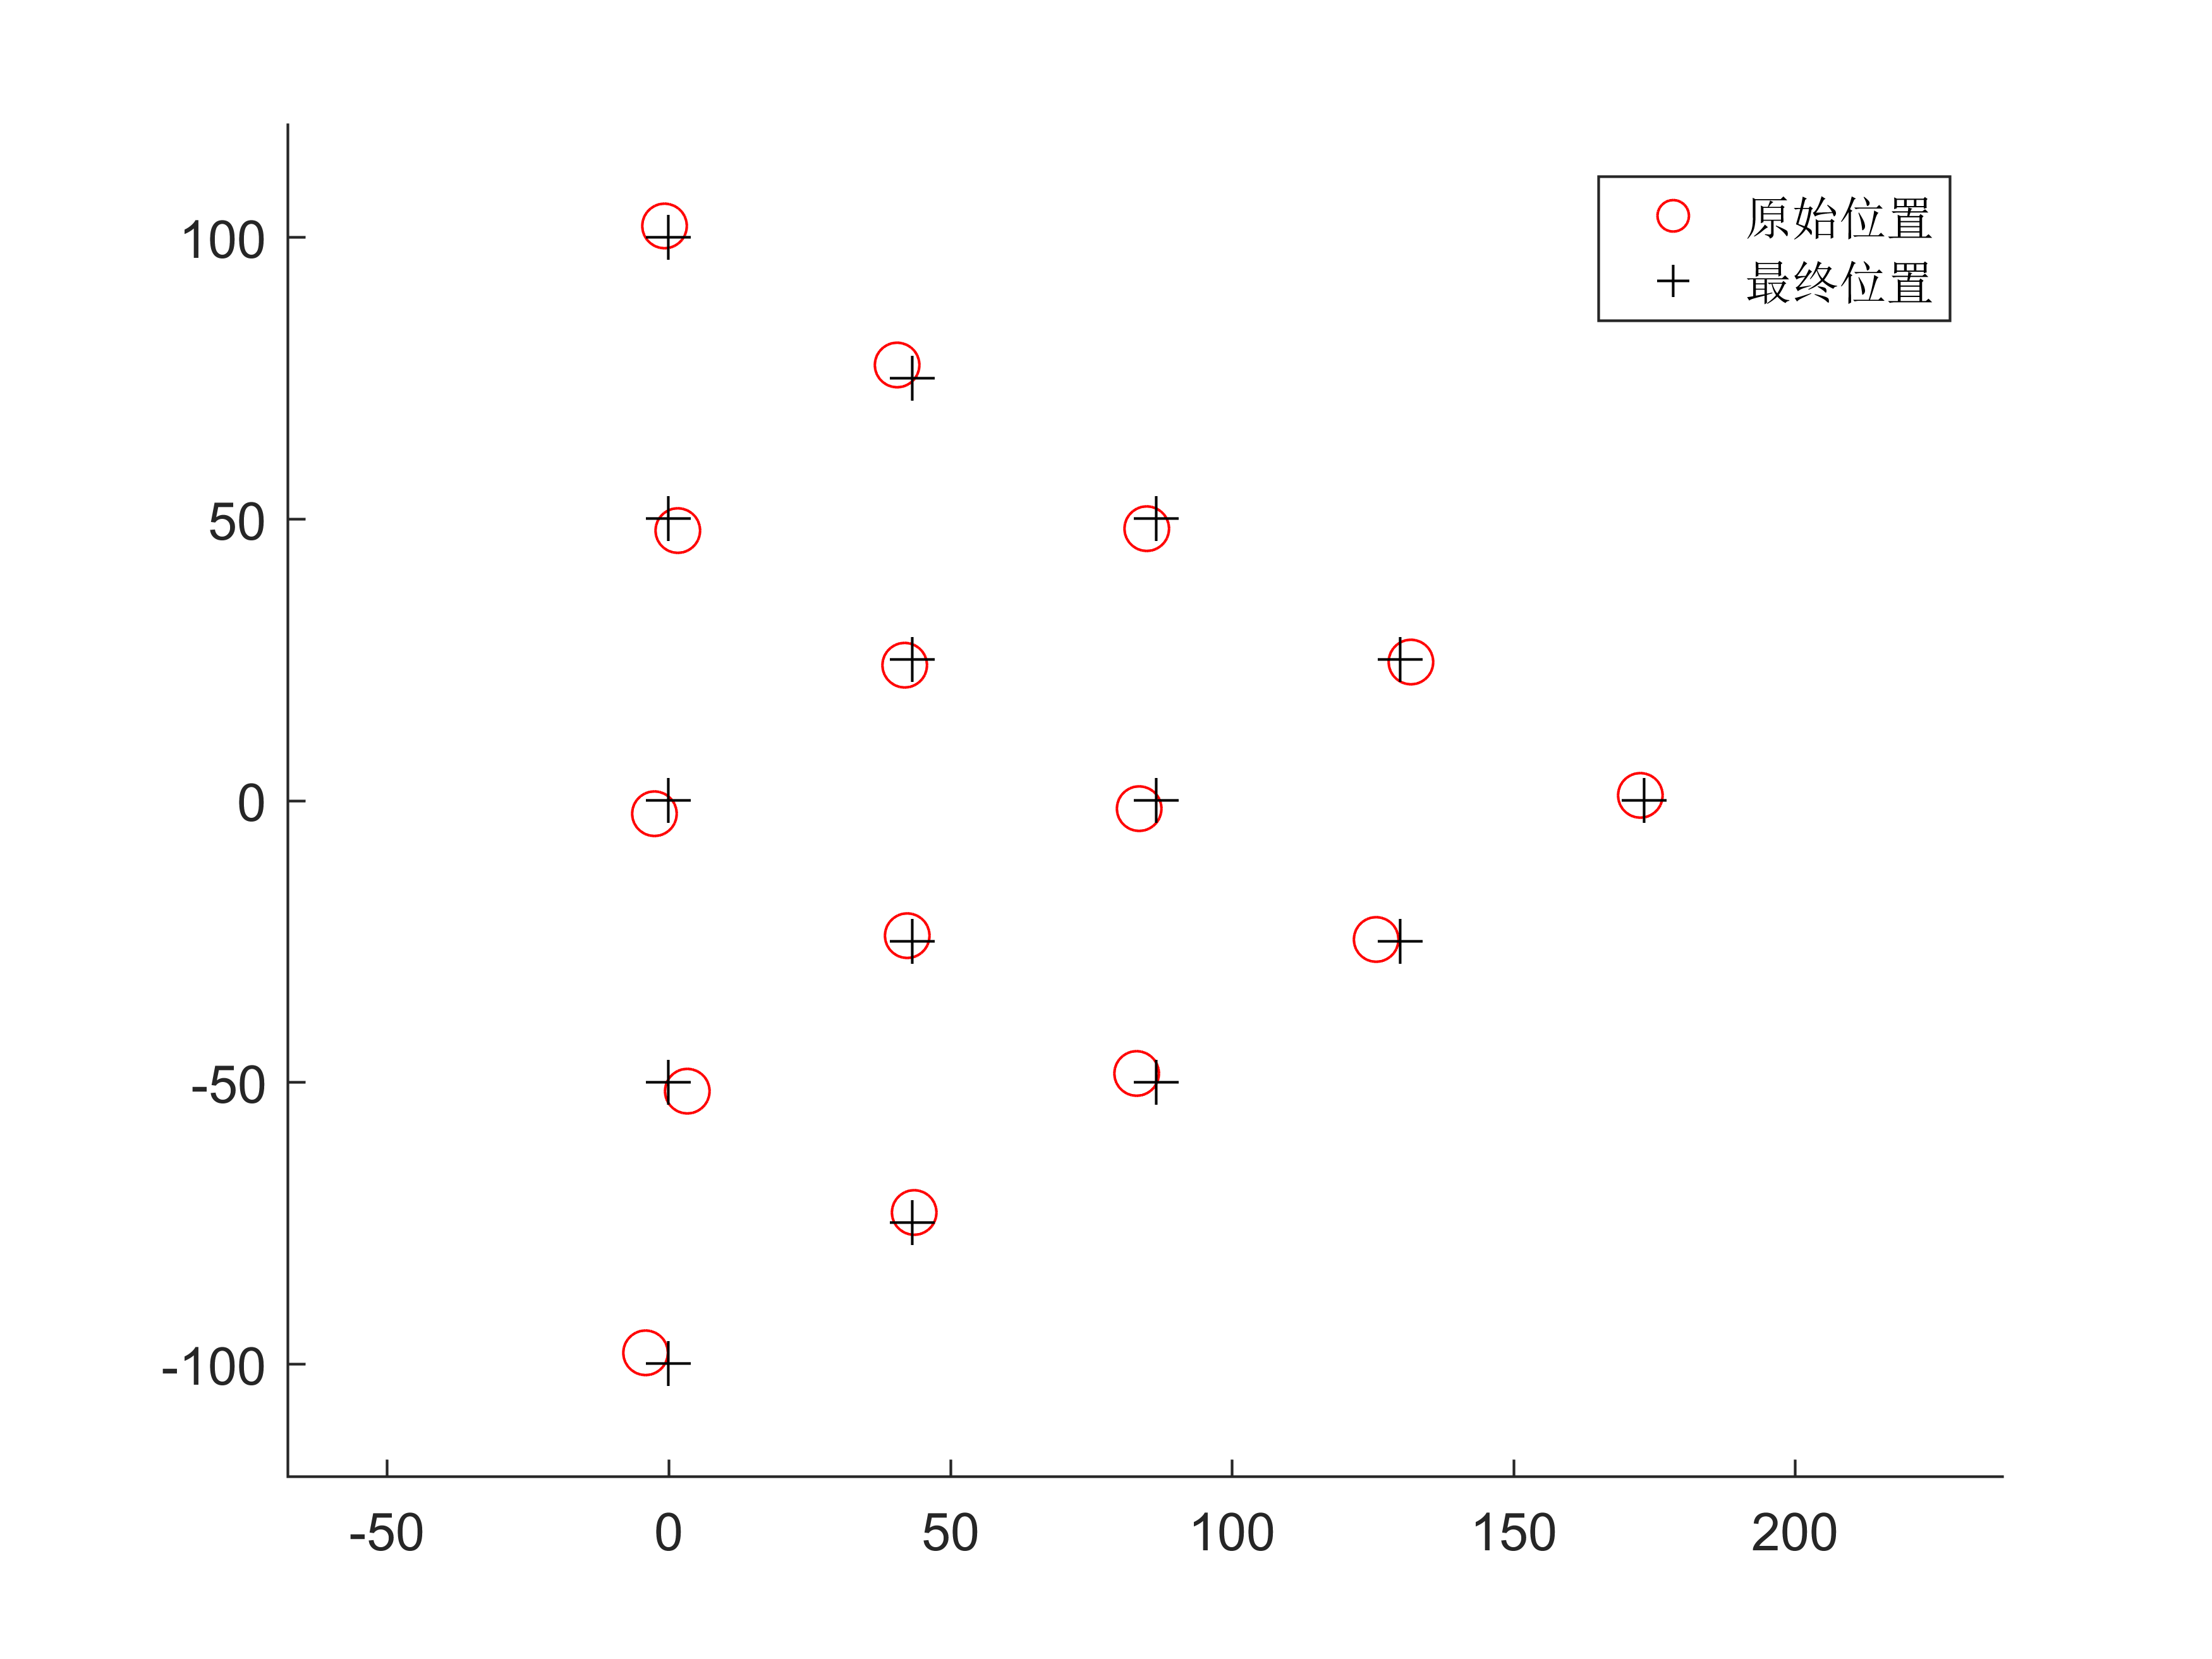
\includegraphics[width=.8\textwidth]{p13}
		\subcaption{无人机调整前后位置图}
		\label{fig:p-12}
	\end{minipage}
	
	\caption{模型求解结果}
\end{figure}

如\cref{fig:p-12}所示,此模型对于无人机位置的调整效果好,且进行十轮位置调整便满足实际需要。

\section{模型的评价与推广}

\subsection{模型优点}
1.问题一第(1)(2)问可以准确的表示出所需要定位的无人机的坐标。

2. 问题一第(3)问的模型基于偏差进行定位,能更好的找到最优半径进行调度,且该模型收敛速度快,效果好。

3.问题一第(3)问及问题2可以对任意要求的飞机编队的半径进行调整与修改,即可以根据实际要求规划目标机群的半径。

4.对于无人机队形的模型建立及优化对于其他编队的情况可以直接进行思想的迁移,即目标函数都为求解误差最小的标准位置并对无人机群进行调整 。

\subsection{模型缺点}
1.由于专业知识的欠缺以及题目假设条件导致的简化,本文建立的模型无法完全模拟无人机在实际飞行过程中由于速度、方向等所造成的位置调整情况。

2.无人机在实际飞行时如果不能向地面发射信号需考虑其高度的误差,本模型在符合题目实际背景的前提下没有对高度差问题进行推广。

\subsection{模型推广}
1.设计其他编队队形的无人机位置调整模型时,可以多分析几种队形,增加模型的普适性。

2.在各个模型的设计时,可以加入时间、速度、高度等因素。
\section{参考文献}
\begin{thebibliography}{9}%宽度9
	\bibitem[1]{22}
	Y. Zeng, R. Zhang and T. J. Lim,
	\newblock "Wireless communications with unmanned aerial vehicles: opportunities and challenges," in IEEE Communications Magazine,
	%\allowbreak[D].
	\newblock vol. 54, no. 5, pp. 36-42, May 2016, doi: 10.1109/MCOM.2016.7470933.
	\bibitem[2]{11}
	林倩玉.
	\newblock 多无人机协同编队控制算法研究\allowbreak[D].
	\newblock 哈尔滨工业大学,2018.


\end{thebibliography}


\newpage
%附录
\begin{appendices}
	\section{支撑材料列表}
	问题一第(3)问
	
	\quad \quad 	\quad \quad 代码
	
	\quad \quad \quad \quad \quad \quad arrs.mat 
	
	\quad \quad \quad \quad \quad \quad kOperate.m 
		
	\quad \quad \quad \quad \quad \quad plot3Circle.m 
			
	\quad \quad \quad \quad \quad \quad plotPositions.m 
				
	\quad \quad \quad \quad \quad \quad polorToXYZ.m 
					
	\quad \quad \quad \quad \quad \quad q3Simulate.m 
						
	\quad \quad \quad \quad \quad \quad xyzToPolor.m 
	
	\quad \quad \quad \quad 数据
							
	\quad \quad \quad \quad \quad \quad 无人机最优调度方案1.xlsx 
	
	\quad \quad \quad \quad \quad \quad 第一轮模拟结果1.xlsx
	
	问题二
	
	\quad \quad 	\quad \quad 代码
	
	\quad \quad \quad \quad \quad \quad deleteNoNeedFromCms.m
	
	\quad \quad \quad \quad \quad \quad getConicalPlanesPos.m 
	
	\quad \quad \quad \quad \quad \quad etRandConPlanePos.m 
	
	\quad \quad \quad \quad \quad \quad plotPositionsConinal.m 
	
	\quad \quad \quad \quad \quad \quad q4Solve.m 
	
	\quad \quad \quad \quad 数据
	
	\quad \quad \quad \quad \quad \quad 无人机最优调度方案2.xlsx 
	
	\quad \quad \quad \quad \quad \quad 第一轮模拟结果2.xlsx
	\section{相关数据}
	\begin{table}[H]
		\caption{问题一第(3)问无人机最终位置坐标}\label{tab:3} \centering
		\begin{tabular}{ccc}
			\toprule[1.5pt]
			\makebox[0.25\textwidth][c]{无人机编号}	&  \makebox[0.25\textwidth][c]{极角$\theta$}& \makebox[0.25\textwidth][c]{极径$\rho$}\\
			
			\midrule[1pt]
			FT00 & 0 & 0\\
			FY01 &0 &  104.63\\
			FY02 & 40 & 104.63\\
			FY03 & 80 &  104.63\\ 
			FY04 & 120 & 104.63\\
			FY05 & 160 & 104.63\\
			FY06 & 200 &  104.63\\
			FY07 & 240 &  104.63 \\
			FY08 & 280 & 104.63\\
			FY09 & 320 &  104.63\\
			
			\bottomrule[1.5pt]
		\end{tabular}
	\end{table}	

\begin{table}[H]
	\caption{问题二无人机初始位置坐标}\label{tab:4} \centering
	\begin{tabular}{ccc}
		\toprule[1.5pt]
		\makebox[0.25\textwidth][c]{无人机编号}	&  \makebox[0.25\textwidth][c]{x}& \makebox[0.25\textwidth][c]{y}\\
		\midrule[1pt]
		FY01&172.49&	0.85\\
		FY02&131.81&24.59\\
		FY03&125.57&	-24.71\\
		FY04&84.89&	48.20\\
		FY05&83.54&	-1.51\\
		FY06&83.07&	-48.50\\
		FY07&40.58&	77.34\\
		FY08&41.96&	24.07\\
		FY09&42.41&	-24.04\\
		FY10&43.64&	-73.12\\
		FY11&-0.7&	101.97\\
		FY12&1.6&	47.93\\
		FY13&-2.56&	-2.30\\
		FY14&3.27&	-51.65\\
		FY15&-4.09&	-98.11\\
		
		\bottomrule[1.5pt]
	\end{tabular}
\end{table}	
	\begin{table}[H]
	\caption{问题二无人机最终位置坐标}\label{tab:5} \centering
	\begin{tabular}{ccc}
		\toprule[1.5pt]
		\makebox[0.25\textwidth][c]{无人机编号}	&  \makebox[0.25\textwidth][c]{x}& \makebox[0.25\textwidth][c]{y}\\
		
		\midrule[1pt]
		FY01&173.20&	0.00\\
		FY02&129.90&	25.00\\
		FY03&129.90&	-25.00\\
		FY04&86.60&	50.01\\
		FY05&86.60&	0.00\\
		FY06&86.60&	-50.00\\
		FY07&43.30&	75.01\\
		FY08&43.30&	25.00\\
		FY09&43.30&	-25.00\\
		FY10&43.30&	-75.00\\
		FY11&0.00&	100.01\\
		FY12&0.00&	50.01\\
		FY13&0.00&	0.00\\
		FY14&0.00&	-50.00\\
		FY15&0.00&	-100.00\\
		
		\bottomrule[1.5pt]
	\end{tabular}
\end{table}	
%	\begin{table}[htbp]
%		\centering
%		\caption{宏包罗列}
%		\begin{tabular}{ccccc}
%			\toprule
%			\multicolumn{5}{c}{模板中已经加载的宏包} \\
%			\midrule
%			amsbsy & amsfonts & {amsgen} & {amsmath} & {amsopn} \\
%			amssymb & amstext & {appendix} & {array} & {atbegshi} \\
%			atveryend & auxhook & {bigdelim} & {bigintcalc} & {bigstrut} \\
%			bitset & bm    & {booktabs} & {calc} & {caption} \\
%			caption3 & CJKfntef & {cprotect} & {ctex} & {ctexhook} \\
%			ctexpatch & enumitem & {etexcmds} & {etoolbox} & {everysel} \\
%			expl3 & fix-cm & {fontenc} & {fontspec} & {fontspec-xetex} \\
%			geometry & gettitlestring & {graphics} & {graphicx} & {hobsub} \\
%			hobsub-generic & hobsub-hyperref & {hopatch} & {hxetex} & {hycolor} \\
%			hyperref & ifluatex & {ifpdf} & {ifthen} & {ifvtex} \\
%			ifxetex & indentfirst & {infwarerr} & {intcalc} & {keyval} \\
%			kvdefinekeys & kvoptions & {kvsetkeys} & {l3keys2e} & {letltxmacro} \\
%			listings & longtable & {lstmisc} & {ltcaption} & {ltxcmds} \\
%			multirow & nameref & {pdfescape} & {pdftexcmds} & {refcount} \\
%			rerunfilecheck & stringenc & {suffix} & {titletoc} & {tocloft} \\
%			trig  & ulem  & {uniquecounter} & {url} & {xcolor} \\
%			xcolor-patch & xeCJK & {xeCJKfntef} & {xeCJK-listings} & {xparse} \\
%			xtemplate & zhnumber &       &       &  \\
%			\bottomrule
%		\end{tabular}%
%		\label{tab:addlabel}%
%	\end{table}%
%	
%	以上宏包都已经加载过了,不要重复加载它们。
	
	\section{问题一第(3)问代码}
	
	\begin{lstlisting}[language=matlab]
	kOperate.m
		function [theta] = kOperate(theta)
		% 保证theta在0-180度中
		theta = abs(theta);
		theta = min(360-theta, theta);
		end
		
	plot3Circle.m
		% 绘制三圆
		rou = 20;
		a = [rou,40];
		b = [rou,160];
		c = [rou,280];
		
		% 未知点
		M = [rou+10,130];
		
		ad = polorToXYZ(a);  bd = polorToXYZ(b); cd = polorToXYZ(c); Md = polorToXYZ(M);
		od = [0,0];
		
		%plot circle
		% viscircles([0 0],rou,'Color','b');%圆心坐标为(0,0),半径为100,轮廓颜色为蓝色
		axis equal
		% set(gca,'XLim',[-30 30]);
		% set(gca,'YLim',[-30 30]);
		hold on
		%% plot 直线
		% %am
		% plot([ad(1),Md(1)], [ad(2),Md(2)], 'k','linewidth',2);
		% %bm
		% plot([bd(1),Md(1)], [bd(2),Md(2)], 'k','linewidth',2);
		% %cm
		% plot([cd(1),Md(1)], [cd(2),Md(2)],'k','linewidth',2);
		% 
		% %ao
		% plot([ad(1),0], [ad(2),0],'k','linewidth',2);
		% %bo
		% plot([bd(1),0], [bd(2),0],'k','linewidth',2);
		% %co
		% plot([cd(1),0], [cd(2),0],'k','linewidth',2);
		% 
		% %mo
		% plot([Md(1),0], [Md(2),0],'k','linewidth',2);
		
		% 画外接圆
		plotOutTri([ad;od;Md])
		plotOutTri([bd;od;Md])
		plotOutTri([cd;od;Md])
		
	plotOutTri.m
		function plotOutTri(p)
		% p=rand(3,2);%(x,y)
		
		cen1=(p(1,:)+p(2,:))/2;         %三角形一条边中点
		cen2=(p(2,:)+p(3,:))/2;         %另一条边中点
		
		k1=-1/((p(1,2)-p(2,2))/(p(1,1)-p(2,1)));    %一条边垂直平分线
		b1=cen1(2)-k1*cen1(1);
		
		k2=-1/((p(2,2)-p(3,2))/(p(2,1)-p(3,1)));    %另一条边垂直平分线
		b2=cen2(2)-k2*cen2(1);
		
		x0=-(b1-b2)/(k1-k2);             %求两直线交点
		y0=-(-b2*k1+b1*k2)/(k1-k2);
		
		r=sqrt((y0-p(1,2))^2+(x0-p(1,1))^2); 
		
		hold on;
		% plot(p(:,1),p(:,2));
		p=circshift(p,1);
		% plot(p(:,1),p(:,2));
		
		theta=0:0.01:2*pi;
		x=x0+r*cos(theta);
		y=y0+r*sin(theta);
		plot(x,y,'-',x0,y0,'.','linewidth',2);
		axis equal
		end
		
	plotPositions.m
		% 绘画positions
		% pos = [[100,0;102.947370926424,40.9878215447839;104.701621875316,79.7685766852877;
		105,119.750000000000;101.584229317453,159.399501370066;108.092849067949,
		199.397185466715;105.000000000000,240.070000000000;102.181496909929,279.878588984783;
		107.503207550062,320.932826590393]];
		
		function plotPositions(pos)
		clf
		rou = mean(pos(:,1));
		
		set(gca,'XLim',[-120 120]);
		set(gca,'YLim',[-120 120]);
		
		% 画圆
		viscircles([0 0],rou,'Color','b','linewidth',1);%圆心坐标为(0,0),半径为100,轮廓颜色为蓝色
		hold on;
		
		x = [0];
		y = [0];
		
		for i=1:size(pos,1)
		tmp = polorToXYZ(pos(i,:));
		x(i+1) = tmp(1);
		y(i+1) = tmp(2);
		end
		
		scatter(x,y,'k');
		plot([x(2:end),x(2)],[y(2:end),y(2)],'r');
		axis equal
		drawnow;
		
		end
		
	polorToXYZ.m
		function [P] = polorToXYZ(p)
		P = zeros(1,2);
		rou = p(1); theta = p(2);
		x = rou*cosd(theta);
		y = rou*sind(theta);
		P(1) = x; P(2) = y;
		end
			
	q3Simulate.m
		%% QuestionⅢ模拟
		clear
		
		% 原始位置1-9 共10台机
		pos = [100, 0;
		98, 40.10;
		112, 80.21;
		105, 119.75;
		98, 159.86;
		112, 199.96;
		105, 240.07;
		98, 280.17;
		112, 320.28
		];
		
		% rng(1);
		% % 误差20%
		% 
		% stdpos = [100, 0;
		% 100, 40;
		% 100, 80;
		% 100, 120;
		% 100, 160;
		% 100, 200;
		% 100, 240;
		% 100, 280;
		% 100, 320
		% ];   
		% 
		% pos = stdpos + rand(size(stdpos))*40-20;
		% pos(pos(:,2)<0,2) = pos(pos(:,2)<0,2) + 360;
		
		% 选择三台机
		arr = [3,6,9];
		
		% 移动系数 lmd1,lmd2 from 0to1
		lmd1 = 1;
		lmd2 = 1;
		lmd = [lmd1, lmd2];
		
		%% 排列
		% arrs = combntns([1:9],3);
		load('arrs.mat');  % arrs 84*3
		
		%% 总运行次数
		total_arr_num = 84;
		plane_num = 9;
		
		%% 迭代次数
		maxIter = 20;
		
		% 变量preset
		res_planeses = zeros(maxIter, length(arr));
		res_errores = zeros(maxIter,1);
		res_positiones = cell(maxIter,1);
		res_detail_errorses = zeros(maxIter,plane_num);
		
		for iter = 1:maxIter
		iter
		total_dises = zeros(total_arr_num,plane_num);
		positionses = cell(total_arr_num,1);
		%% 调用代码开始模拟
		for j=1:total_arr_num
		% j = 1;
		arr = arrs(j,:);
		
		[dises, positions] = simulateArr(arr,lmd, pos);
		
		total_dises(j,:) = dises';
		positionses{j} = positions;
		end
		
		sum_dises = sum(total_dises,2);
		%% 单次结束后,第j个组合
		[~, index] = sort(sum_dises,'ascend');
		first_ind = index(1);
		% 结果飞机调度,总误差,最后飞机位置,误差细节
		res_planes = arrs(first_ind,:);
		res_error = sum_dises(first_ind);
		res_position = positionses{first_ind};
		res_detail_errors = total_dises(first_ind,:);
		
		res_planeses(iter,:) = res_planes;
		res_errores(iter) = res_error;
		res_positiones{iter} = res_position;
		res_detail_errorses(iter,:) = res_detail_errors;
		
		pos = res_position;
		
		plotPositions(pos);
		
		end
		
		figure();
		plot(res_errores);
		
		function [dises, positions] = simulateArr(arr, lmd, pos)
		
		% 理想角 (360/9)
		I_Angles = [0,40,80,120,160,200,240,280,320];
		
		% 理想rou
		rou = 100;
		
		% 飞机个数
		plane_num = 9;
		
		% % 原始位置1-9 共10台机
		% pos = [100, 0;
		% 98, 40.10;
		% 112, 80.21;
		% 105, 119.75;
		% 98, 159.86;
		% 112, 199.96;
		% 105, 240.07;
		% 98, 280.17;
		% 112, 320.28
		% ];
		
		dises = zeros(plane_num,1);
		
		positions = zeros(plane_num, 2);
		
		p_T_rou = mean(pos(:,1));
		
		% % 测试固定半径
		% p_T_rou = 110;
		
		%
		for i=1:plane_num
		
		%% 开始运算
		% i = 3;
		p_R = pos(i,:);   % 当前实际位置(极坐标)
		
		%% 计算当前位置
		p_C = zeros(1,2);   % 当前计算位置(极坐标)
		p_C(2) = p_R(2);    % theta'' = theta';
		
		theta_R = p_R(2);
		
		% 第几台机,存在精度误差,取中位数
		rou_cs = zeros(3,1);
		
		for k=1:length(arr)
		indArrPlane = k;
		% 求解alphaA和thetaA
		thetaA = I_Angles(arr(indArrPlane));
		
		% 测试利用全圆定位通过
		% 用实际飞机定位,利用向量积求角(先转为平面直角坐标)
		ARealPos = pos(arr(indArrPlane),:); % 极坐标
		OPos = [0,0];
		AM = polorToXYZ(p_R) - polorToXYZ(ARealPos);
		OM = polorToXYZ(p_R) - polorToXYZ(OPos);
		sigma = acos(dot(AM,OM)/(norm(AM)*norm(OM)));
		alphaA = sigma*180/pi;
		
		% 求解rou'
		rou_c_coe = sind(kOperate(thetaA - theta_R) + alphaA)/sind(alphaA);
		rou_c = rou*rou_c_coe;
		
		rou_cs(k) = rou_c;
		end
		rou_c = median(rou_cs);
		
		p_C(1) = rou_c;
		
		%% step2 计算 当前位置与假性理想位置差 (直角坐标)
		p_FK = [rou, I_Angles(i)];
		
		% 位置差(直角坐标)
		p_D = polorToXYZ(p_FK) - polorToXYZ(p_C);
		
		% 乘上移动系数
		p_D = lmd.*p_D;
		
		%% step3 换算到当前位置下p_R(即进行移动)
		p_R_XYZ = polorToXYZ(p_R);
		
		% 若是调度的飞机则不移动
		if ismember(i,arr)
		p_R_XYZ = polorToXYZ(p_R);
		else
		p_R_XYZ = p_R_XYZ + p_D;
		end
		
		p_R_after = xyzToPolor(p_R_XYZ);
		
		clear TH R
		
		%% step4 计算与真实理想位置
		% 计算真实理想位置
		p_T_polor = [p_T_rou, I_Angles(i)];
		p_T_XYZ = polorToXYZ(p_T_polor);
		
		% 计算距离
		dis = sqrt(sum((p_R_XYZ - p_T_XYZ).^2));
		
		% 赋值
		dises(i) = dis;
		positions(i,:) = p_R_after;
		end
		%
		
		end
		
	xyzToPolor.m
		function p = xyzToPolor(p_xyz)
		p = zeros(1,2);
		[TH, R]= cart2pol(p_xyz(1),p_xyz(2));
		p(1) = R;
		p(2) = TH*180/pi;
		if p(2) < 0
		% 为负则变成正
		p(2) = 360 + p(2);
		end
		
		end
		
		
	\end{lstlisting}
	
	\section{问题二代码}
	
	\begin{lstlisting}[language=matlab]
	deleteNoNeedFromCms.m	
		clear
		% 鉴别组合和不需要的
		noneed = [1	2	3
		1	4	6
		1	7	10
		1	11	15
		1	12	14
		1	8	9
		5	2	3
		5	4	6
		5	7	10
		5	11	15
		5	12	14
		5	8	9
		];
		
		
		
		need_plans_plane = [1,2,3,4,5,6,7,8,9,10,11,12,14,15];
		
		arrs = combntns(need_plans_plane,3);
		newArrs = [];
		k = 1;
		flag = true;
		
		for j = 1:size(arrs,1)
		flag = true;
		for i = 1:size(noneed,1)
		if sum(sort(noneed(i,:))==sort(arrs(j,:))) == 3
		% 存在了
		flag = false;
		end
		end
		if flag == true
		% 添加
		newArrs(k,:) = arrs(j,:);
		k = k+1;
		end
		end
		arrs = newArrs;
		
	plotPositionsConinal.m
		function [position] = getConicalPlanesPos(number)
		% 返回锥形所处位置i的飞机
		X = [
		4,0;
		3,1;
		3,-1;
		2,2;
		2,0;
		2,-2;
		1,3;
		1,1;
		1,-1;
		1,-3;
		0,4;
		0,2;
		0,0;
		0,-2;
		0,-4];
		position = X(number,:);
		end
		
	getRandConPlanePos.m
		function [position] = getRandConPlanePos(number)
		% 获取飞机真实位置
		% 误差1%内
		ratio = 0.01;
		X = [
		4,0;
		3,1;
		3,-1;
		2,2;
		2,0;
		2,-2;
		1,3;
		1,1;
		1,-1;
		1,-3;
		0,4;
		0,2;
		0,0;
		0,-2;
		0,-4];
		X = X + rand(size(X))*ratio*2-ratio;  %[-0.05,0.05];
		position = X(number,:);
		end
		
	plotPositionsConinal.m
		% 绘画positions
		% pos = [[100,0;102.947370926424,40.9878215447839;104.701621875316,79.7685766852877;105,119.750000000000;101.584229317453,159.399501370066;108.092849067949,199.397185466715;105.000000000000,240.070000000000;102.181496909929,279.878588984783;107.503207550062,320.932826590393]];
		function plotPositionsConinal(pos)
		% clf
		% rou = mean(pos(:,1));
		
		
		
		% x = [0];
		% y = [0];
		
		% for i=1:size(pos,1)
		%     x(i) = tmp(1);
		%     y(i) = tmp(2);
		% end
		
		x = pos(:,1)';
		y = pos(:,2)';
		
		scatter(x,y,72,'k+');
		set(gca,'XLim',[-120 120]);
		set(gca,'YLim',[-120 120]);
		% plot([x(1:end),x(1)],[y(1:end),y(1)],'r');
		axis equal
		% drawnow;
		
		end
		
	q4Slove.m
		%% q4 求解
		clear
		ratio = 0.1;
		sdPos = [
		4,0;
		3,1;
		3,-1;
		2,2;
		2,0;
		2,-2;
		1,3;
		1,1;
		1,-1;
		1,-3;
		0,4;
		0,2;
		0,0;
		0,-2;
		0,-4];
		
		rdPos = sdPos + rand(size(sdPos))*ratio*2-ratio;  %[-0.05,0.05];
		
		% 间距
		sigma = 50;
		
		new_sigma = 45;  % 固定间距
		
		plane_num = 14;
		% new_sigma = 45;  % 新间距
		
		lmd = [1,1];
		arr = [2,6,7];
		
		%% 实际计算
		rng(1);
		
		onex = sqrt(3)/2;
		oney = 1/2;
		std_cords = [onex, oney];
		
		% std and new
		cords = sigma * std_cords;
		new_cords = new_sigma * std_cords;
		
		sdIdealpos = sdPos.*cords;
		pos = rdPos.*cords;
		
		
		dises = zeros(plane_num,1);
		positions = zeros(plane_num, 2);
		%plane number
		
		need_plans_plane = [1,2,3,4,5,6,7,8,9,10,11,12,14,15];
		
		% arrs = combntns(need_plans_plane,3);
		load('arrsQ4.mat');
		total_arr_num = size(arrs,1);
		
		%% 迭代次数
		maxIter = 50;
		
		% 变量preset
		res_planeses = zeros(maxIter, length(arr));
		res_errores = zeros(maxIter,1);
		res_positiones = cell(maxIter,1);
		res_detail_errorses = zeros(maxIter,plane_num);
		
		for iter = 1:maxIter
		iter
		total_dises = zeros(total_arr_num,plane_num);
		positionses = cell(total_arr_num,1);
		
		for arrt=1:total_arr_num
		arr = arrs(arrt,:);
		
		
		for i = 1:plane_num
		% 共14架
		pn = need_plans_plane(i);
		
		% pn = 8;
		
		
		
		O = [0,0];
		%标准机位置
		% 4
		sdA = sdIdealpos(arr(1),:);
		% 7
		sdB = sdIdealpos(arr(2),:);
		% 6
		sdC = sdIdealpos(arr(3),:);
		
		% 偏移后
		A = pos(arr(1),:);
		B = pos(arr(2),:);
		C = pos(arr(3),:);
		
		
		M = pos(pn,:);
		
		%% 求解直线参数
		% A,B
		[la_params(1),la_params(2)] = solveAB(M,A);
		[lb_params(1),lb_params(2)] = solveAB(M,B);
		[lc_params(1),lc_params(2)] = solveAB(M,C);
		
		% C
		la_C = -la_params(1)*sdA(1) - la_params(2)*sdA(2);
		lb_C = -lb_params(1)*sdB(1) - lb_params(2)*sdB(2);
		lc_C = -lc_params(1)*sdC(1) - lc_params(2)*sdC(2);
		
		
		[xab,yab] = solveLineInsect([la_params,la_C], [lb_params,lb_C]);
		[xbc,ybc] = solveLineInsect([lb_params,lb_C], [lc_params,lc_C]);
		[xac,yac] = solveLineInsect([la_params,la_C], [lc_params,lc_C]);
		
		% 用边界做初始值
		x0 = [xac,yac];
		
		params = [la_params;lb_params;lc_params];  %3*2
		Ces = [la_C,lb_C,lc_C];
		
		noteqcons = x0*params' + Ces ;    %1*3 <=0
		
		% 标准点集合
		sdPoints = [sdA;sdB;sdC];
		% 标准alpha
		alphaA = calAlpha(A,M,O);
		alphaB = calAlpha(B,M,O);
		alphaC = calAlpha(C,M,O);
		alphas = [alphaA,alphaB,alphaC];
		
		X_tmp = [xab,yab;xbc,ybc;xac,yac];
		X_tmp = [X_tmp;mean(X_tmp(:,1)),mean(X_tmp(:,2))];
		tmp_err = zeros(4,1);
		for j=1:4
		tmp_err(i) = cosError(X_tmp(j,:),sdPoints,alphas);
		end
		[~,ind] = sort(tmp_err,'ascend');
		first_ind = ind(1);
		res = X_tmp(first_ind,:);
		fval = tmp_err(first_ind);
		% inital_error = cosError(x0,sdPoints,alphas);
		% 
		% fun = @(X)cosError(X,sdPoints,alphas);
		% conFun = @(X)unlinearC(X,params,Ces);
		% 
		% options = optimset('Algorithm','sqp');
		% [res,fval] = fmincon(fun,x0,[],[],[],[],[],[],conFun,options);
		
		% % % 画图查看点和区域分布
		% plot([xab,xbc,xac,xab],[yab,ybc,yac,yab]);
		% hold on;
		% scatter(res(1),res(2));
		
		%% res为计算距离,要移动到目标位置
		p_FI = sdIdealpos(pn,:);
		p_R = M;
		p_C = res;
		p_T = sdIdealpos(pn,:);
		
		%% 移动向量
		p_D = p_FI - p_C;
		
		p_D = lmd .* p_D;  % 控制移动步长
		
		
		%% 飞机移动
		% 若是调度的飞机则不移动
		if ismember(pn,arr)
		p_R_after = p_R;
		else
		p_R_after = p_R + p_D;
		end
		
		% 计算误差
		dis = sqrt(sum((p_R_after - p_T).^2));
		
		% 赋值
		dises(i) = dis;
		positions(i,:) = p_R_after;
		
		end
		
		total_dises(arrt,:) = dises';
		positionses{arrt} = positions;
		
		end
		
		sum_dises = sum(total_dises,2);
		%% 单次结束后,第j个组合
		[~, index] = sort(sum_dises,'ascend');
		first_ind = index(1);
		% 结果飞机调度,总误差,最后飞机位置,误差细节
		res_planes = arrs(first_ind,:);
		res_error = sum_dises(first_ind);
		res_position = positionses{first_ind};
		res_detail_errors = total_dises(first_ind,:);
		
		res_planeses(iter,:) = res_planes;
		res_errores(iter) = res_error;
		res_positiones{iter} = res_position;
		res_detail_errorses(iter,:) = res_detail_errors;
		
		% pos = res_position;
		% 添加原点
		pos(1:12,:) = res_position(1:12,:);
		pos(14:15,:) = res_position(13:14,:);
		pos(13,:) = [0,0];
		
		plotPositionsConinal(pos);
		end
		
		figure();
		plot(res_errores);
		
		function [c,ceq] = unlinearC(X,params,Ces)
		% X(x0,y0)
		ctmp = X*params' + Ces ;  % 1*3 <=0
		c = prod(ctmp);   %1*1 <=0
		ceq = [];
		end
					
	\end{lstlisting}
\end{appendices}


%
%\section{模板的基本使用}
%
%
%根据要求,电子版论文提交时需去掉封面和编号页。可以加上 \verb|withoutpreface|  选项来实现,即:
%\begin{tcode}
%    \documentclass[withoutpreface]{cumcmthesis}
%\end{tcode}
%这样就能实现了。打印的时候有超链接的地方不需要彩色,可以加上 \verb|bwprint| 选项。
%
%另外目录也是不需要的,将 \verb|\tableofcontents| 注释或删除,目录就不会出现了。
%
%团队的信息填入指定的位置,并且确保信息的正确性,以免因此白忙一场。
%
%编译记得使用 \verb|xelatex|,而不是用 \verb|pdflatex|。在命令行编译的可以按如下方式编译:
%\begin{tcode}
%	xelatex example
%\end{tcode}
%或者使用 \verb|latexmk| 来编译,更推荐这种方式。
%\begin{tcode}
%	latexmk -xelatex example
%\end{tcode}
%
%下面给出写作与排版上的一些建议。
%
%\section{图片}
%
%建模中不可避免要插入图片。图片可以分为矢量图与位图。位图推荐使用 \verb|jpg,png| 这两种格式,避免使用 \verb|bmp| 这类图片,容易出现图片插入失败这样情况的发生。矢量图一般有 \verb|pdf,eps| ,推荐使用 \verb|pdf|  格式的图片,尽量不要使用 \verb|eps| 图片,理由相同。
%
%注意图片的命名,避免使用中文来命名图片,可以用英文与数字的组合来命名图片。避免使用\verb|1,2,3| 这样顺序的图片命名方式。图片多了,自己都不清楚那张图是什么了,命名尽量让它有意义。下面是一个插图的示例代码。
%\begin{figure}[!h]
%    \centering
%    \includegraphics[width=.6\textwidth]{smokeblk}
%    \caption{电路图}
%    \label{fig:circuit-diagram}
%\end{figure}
%
%注意 \verb|figure| 环境是一个浮动体环境,图片的最终位置可能会跑动。\verb|[!h]| 中的 \verb|h| 是 here 的意思, \verb|!| 表示忽略一些浮动体的严格规则。另外里面还可以加上 \verb|btp| 选项,它们分别是 bottom, top, page 的意思。只要这几个参数在花括号里面,作用是不分先后顺序的。page 在这里表示浮动页。
%
%\verb|\label{fig:circuit-diagram}| 是一个标签,供交叉引用使用的。例如引用图片 \verb|\cref{fig:circuit-diagram}| 的实际效果是 \cref{fig:circuit-diagram}。图片是自动编号的,比起手动编号,它更加高效。\verb|\cref{label}| 由 \verb|cleveref| 宏包提供,比普通的 \verb|\ref{label}| 更加自动化。 \verb|label| 要确保唯一,命名方式推荐用图片的命名方式。
%
%图片并排的需求解决方式多种多样,下面用 \verb|minipage| 环境来展示一个简单的例子。注意,以下例子用到了 \verb|subcaption| 命令,需要加载 subcaption 宏包。
%
%\begin{figure}
%    \centering
%    \begin{minipage}[c]{0.3\textwidth}
%        \centering
%        \includegraphics[width=0.95\textwidth]{f1}
%        \subcaption{流程图}
%        \label{fig:sample-figure-a}
%    \end{minipage}
%    \begin{minipage}[c]{0.3\textwidth}
%        \centering
%        \includegraphics[width=0.95\textwidth]{f1}
%        \subcaption{流程图}
%        \label{fig:sample-figure-b}
%    \end{minipage}
%    \begin{minipage}[c]{0.3\textwidth}
%        \centering
%        \includegraphics[width=0.95\textwidth]{f1}
%        \subcaption{流程图}
%        \label{fig:sample-figure-c}
%    \end{minipage}
%    \caption{多图并排示例}
%    \label{fig:sample-figure}
%\end{figure}
%这相当于整体是一张大图片,大图片引用是\cref{fig:sample-figure},子图引用别分是\cref{fig:sample-figure-a}、\cref{fig:sample-figure-b}、\cref{fig:sample-figure-c}。
%
%如果原本两张图片的高度不同,但是希望它们缩放后等高的排在同一行,参考这个例子:
%\begin{figure}
%    \centering
%    \begin{minipage}[c]{0.48\textwidth}
%        \centering
%        \includegraphics[height=0.2\textheight]{cat}
%        \subcaption{一只猫}
%    \end{minipage}
%    \begin{minipage}[c]{0.48\textwidth}
%        \centering
%        \includegraphics[height=0.2\textheight]{smokeblk}
%        \subcaption{电路图}
%    \end{minipage}
%    \caption{多图并排示例}
%\end{figure}

%\section{绘制普通三线表格}
%表格应具有三线表格式,因此常用 booktabs宏包,其标准格式如\cref{tab:001}~所示。
%\begin{table}[!htbp]
%    \caption{标准三线表格}\label{tab:001} \centering
%    \begin{tabular}{ccccc}
%        \toprule[1.5pt]
%        $D$(in) & $P_u$(lbs) & $u_u$(in) & $\beta$ & $G_f$(psi.in)\\
%        \midrule[1pt]
%        5 & 269.8 & 0.000674 & 1.79 & 0.04089\\
%        10 & 421.0 & 0.001035 & 3.59 & 0.04089\\
%        20 & 640.2 & 0.001565 & 7.18 & 0.04089\\
%        \bottomrule[1.5pt]
%    \end{tabular}
%\end{table}
%
%其绘制表格的代码及其说明如下。
%\begin{tcode}
%    \begin{table}[!htbp]
%        \caption[标签名]{中文标题}
%        \begin{tabular}{cc...c}
%            \toprule[1.5pt]
%            表头第1个格   & 表头第2个格   & ... & 表头第n个格  \\
%            \midrule[1pt]
%            表中数据(1,1) & 表中数据(1,2) & ... & 表中数据(1,n)\\
%            表中数据(2,1) & 表中数据(2,2) & ... & 表中数据(2,n)\\
%            ...................................................\\
%            表中数据(m,1) & 表中数据(m,2) & ... & 表中数据(m,n)\\
%            \bottomrule[1.5pt]
%        \end{tabular}
%    \end{table}
%\end{tcode}
%
%\bigskip
%
%table环境是一个将表格嵌入文本的浮动环境。tabular环境的必选参数由每列对应一个格式字符所组成:c表示居中,l表示左对齐,r表示右对齐,其总个数应与表的列数相同。此外,\verb|@{文本}|可以出现在任意两个上述的列格式之间,其中的文本将被插入每一行的同一位置。表格的各行以\verb|\\|分隔,同一行的各列则以\&分隔。 \verb|\toprule| 、\verb|\midrule| 和 \verb|\bottomrule| 三个命令是由booktabs宏包提供的,其中 \verb|\toprule| 和 \verb|\bottomrule| 分别用来绘制表格的第一条(表格最顶部)和第三条(表格最底部)水平线, \verb|\midrule| 用来绘制第二条(表头之下)水平线,且第一条和第三条水平线的线宽为 1.5pt ,第二条水平线的线宽为 1pt 。引用方法与图片的相同。
%
%\section{公式}
%
%数学建模必然涉及不少数学公式的使用。下面简单介绍一个可能用得上的数学环境。
%
%首先是行内公式,例如 $ \theta $ 是角度。行内公式使用 \verb|$  $| 包裹。
%
%行间公式不需要编号的可以使用 \verb|\[  \]| 包裹,例如
%\[
%E=mc^2
%\]
%其中 $ E $ 是能量,$ m $ 是质量,$ c $ 是光速。
%
%如果希望某个公式带编号,并且在后文中引用可以参考下面的写法:
%\begin{equation}
%E=mc^2
%\label{eq:energy}
%\end{equation}
%式\cref{eq:energy}是质能方程。
%
%多行公式有时候希望能够在特定的位置对齐,以下是其中一种处理方法。
%\begin{align}
%P & = UI \\
%& = I^2R
%\end{align}
%\verb|&| 是对齐的位置, \verb|&| 可以有多个,但是每行的个数要相同。
%
%矩阵的输入也不难。
%\[
%\mathbf{X} = \left(
%    \begin{array}{cccc}
%    x_{11} & x_{12} & \ldots & x_{1n}\\
%    x_{21} & x_{22} & \ldots & x_{2n}\\
%    \vdots & \vdots & \ddots & \vdots\\
%    x_{n1} & x_{n2} & \ldots & x_{nn}\\
%    \end{array} \right)
%\]
%
%分段函数这些可以用 \verb|case| 环境,但是它要放在数学环境里面。
%\[
%f(x) =
%    \begin{cases}
%        0 &  x \text{为无理数} ,\\
%        1 &  x \text{为有理数} .
%    \end{cases}
%\]
%在数学环境里面,字体用的是数学字体,一般与正文字体不同。假如要公式里面有个别文字,则需要把这部分放在 \verb|text| 环境里面,即 \verb|\text{文本环境}| 。
%
%公式中个别需要加粗的字母可以用 \verb|$\bm{math symbol}$| 。如 $ \alpha a\bm{\alpha a} $ 
%
%\section{参考文献与引用}
%
%参考文献对于一篇正式的论文来说是必不可少的,在建模中重要的参考文献当然应该列出。\LaTeX{}在这方面的功能也是十分强大的,下面进介绍一个比较简单的参考文献制作方法。有兴趣的可以学习 \verb|bibtex| 或 \verb|biblatex| 的使用。
%
%\LaTeX{}的入门书籍可以看《\LaTeX{}入门》\cite{liuhaiyang2013latex}。这是一个简单的引用,用 \verb|\cite{bibkey}| 来完成。要引用成功,当然要维护好 bibitem 了。下面是个简单的例子。
%
%
%
%%参考文献
%\begin{thebibliography}{9}%宽度9
%    \bibitem[1]{liuhaiyang2013latex}
%    刘海洋.
%    \newblock \LaTeX {}入门\allowbreak[J].
%    \newblock 电子工业出版社, 北京, 2013.
%    \bibitem[2]{mathematical-modeling}
%    全国大学生数学建模竞赛论文格式规范 (2020 年 8 月 25 日修改).
%    \bibitem{3} \url{https://www.latexstudio.net}
%\end{thebibliography}

\end{document} 